\documentclass[nojss]{jss} % nojss articlen sijaan

%\VignetteIndexEntry{uGMAR: A Family of Mixture Autoregressive Models in R}

%% setwd("/Users/savi/Desktop/uGMARartikkeli/jss-article-rnw")
%% Sweave("uGMARpaper.Rnw")
%% tools::texi2pdf("uGMARpaper.tex")

%% -- LaTeX packages and custom commands ---------------------------------------

% Margin setup
\usepackage[margin=1in]{geometry}

%% recommended packages
\usepackage{thumbpdf,lmodern}

%% another package (only for this demo article)
\usepackage{framed}

%% Packages added by the author
\usepackage{amsmath} % \align, etc.
\usepackage{amssymb} % \mathbb, etc.
\usepackage{mathtools} % matrix*: [c] centered, [l] left-aligned, [r] right-aligned

% Adjustwidth environment
\usepackage{changepage}

%% new custom commands
\newcommand{\class}[1]{`\code{#1}'}
\newcommand{\fct}[1]{\code{#1()}}

%% TOC:
\makeatletter
\def\tableofcontents{%
  \section*{\contentsname}%
  \@starttoc{toc}%
}
\makeatother

%% For Sweave-based articles about R packages:
%% need no \usepackage{Sweave}



%% -- Article metainformation (author, title, ...) -----------------------------

%% - \author{} with primary affiliation
%% - \Plainauthor{} without affiliations
%% - Separate authors by \And or \AND (in \author) or by comma (in \Plainauthor).
%% - \AND starts a new line, \And does not.
\author{Savi Virolainen\\ University of Helsinki}
\Plainauthor{Savi Virolainen}

%% - \title{} in title case
%% - \Plaintitle{} without LaTeX markup (if any)
%% - \Shorttitle{} with LaTeX markup (if any), used as running title
%%\title{A Short Demo Article: Regression Models for Count Data in \proglang{R}}
\title{uGMAR: A Family of Mixture Autoregressive Models in \proglang{R}}
\Plaintitle{uGMAR: A Family of Mixture Autoregressive Models in R}
\Shorttitle{A Family of Mixture Autoregressive Models in \proglang{R}}

\Abstract{
We describe the \proglang{R} package \pkg{uGMAR}, which provides tools for estimating and analyzing the Gaussian mixture autoregressive model, the Student's $t$ mixture autoregressive model, and the Gaussian and Student's $t$ mixture autoregressive model. These three models constitute an appealing family of mixture autoregressive models that we call the GSMAR models. The model parameters are estimated with the method of maximum likelihood by running multiple rounds of a two-phase estimation procedure in which a genetic algorithm is used to find starting values for a gradient based method. For evaluating the adequacy of the estimated models, \pkg{uGMAR} utilizes so-called quantile residuals and provides functions for graphical diagnostics as well as for calculating formal diagnostic tests. \pkg{uGMAR} also facilitates simulation from the GSMAR processes and forecasting future values of the process by a simulation-based Monte Carlo method. We illustrate the use of \pkg{uGMAR} with the monthly U.S. interest rate spread between the 10-year and 1-year Treasury rates.
}

%% - \Keywords{} with LaTeX markup, at least one required
%% - \Plainkeywords{} without LaTeX markup (if necessary)
%% - Should be comma-separated and in sentence case.
\Keywords{mixture autoregressive model, regime-switching, Gaussian mixture, Student's $t$ mixture}
\Plainkeywords{mixture autoregressive model, regime-switching, Gaussian mixture, Student's t mixture}

%% - \Address{} of at least one author
%% - May contain multiple affiliations for each author
%%   (in extra lines, separated by \emph{and}\\).
%% - May contain multiple authors for the same affiliation
%%   (in the same first line, separated by comma).
\Address{
  Savi Virolainen\\
  Faculty of Social Sciences\\
  University of Helsinki\\
  P. O. Box 17, FI-0014 University of Helsinki, Finland\\
  E-mail: \email{savi.virolainen@helsinki.fi}
}

\begin{document}

% Table of contents
\pagenumbering{gobble}
\pagebreak
\tableofcontents
\vfill
\pagebreak
\pagenumbering{arabic}

\section{Introduction}
\addcontentsline{toc}{section}{Introduction}

A popular method for modeling univariate time series is to employ a linear autoregressive (AR) model that assumes the process to be generated by a weighted sum of the preceding $p$ observations, an intercept term, and a random error. The error process is often assumed to be serially uncorrelated with zero mean and constant variance. This encompasses conditionally homoskedastic processes, such as independent and identically distributed (IID) processes, as well as conditionally heteroskedastic processes, such as autoregressive conditional heteroskedasticity (ARCH) processes \citep{Engle:1982} and generalized autoregressive conditional heteroskedasticity (GARCH) processes \citep{Bollerslev:1986}.

Several \proglang{R} packages accommodate linear AR modeling with various types of error processes. The \proglang{R} package \pkg{forecast} \citep{Hyndman+Athanasopoulos+Bergmeir+Caceres+Chhay+O'Hara-Wild+Petropoulos+Razbash+Wang+Yasmeen:2021}, for instance, accommodates estimation of AR models with seasonal components. The \proglang{R} package \pkg{fGarch} \citep{Wuertz+Chalabi+Boudt+Chausse+Miklovac:2020}, on the other hand, facilitates estimation of AR models with ARCH and GARCH errors following various distributions, including normal, Student's $t$-, and generalized error distributions and their skewed versions. A more comprehensive set of error processes are provided in the popular \proglang{R} package \pkg{rugarch} \citep{Ghalanos:2020}. It accommodates a rich set of different GARCH processes with several error distributions, including the regular and skewed versions of normal, $t$-, and generalized error distributions, as well as generalized hyperbolic normal and inverse Gaussian distributions, to name a few.

A linear AR model with potentially skewed GARCH errors can often filter the autocorrelation and conditional heteroskedasticity from the series very well. But in some cases, it cannot adequately capture all the relevant characteristics of the series, including
shifts in the mean or volatility, and changes in the dynamics of the process. Such nonlinear features frequently occur in economic time series when the underlying data generating dynamics vary in time, for example, depending on the specific state of the economy.

Various types of time series models capable of capturing such regime-switching behavior have been proposed, one of them being the class of mixture models introduced by \cite{Le+Martin+Raftery:1996} and further developed by, among others, \cite{Wong+Li:2000, Wong+Li:2001, Wong+Li2:2001}, \cite{Glasbey:2001}, \cite{Lanne+Saikkonen:2003}, \cite{Kalliovirta+Meitz+Saikkonen:2015}, \cite{Meitz+Preve+Saikkonen:2021}, and \cite{Virolainen:2020}. Following the recent developments by \cite{Kalliovirta+Meitz+Saikkonen:2015}, \cite{Meitz+Preve+Saikkonen:2021}, and \cite{Virolainen:2020}, we consider the Gaussian mixture autoregressive (GMAR) model, the Student's $t$ mixture autoregressive (StMAR) model, and the Gaussian and Student's $t$ mixture autoregressive (G-StMAR) model. These three models constitute an appealing family of mixture autoregressive models that we call the GSMAR models.

A GSMAR process generates each observation from one of its mixture components, which are either conditionally homoskedastic linear Gaussian autoregressions or conditionally heteroskedastic linear Student's $t$ autoregressions. The mixture component that generates each observation is randomly selected according to the probabilities determined by the mixing weights that, for a $p$th order model, depend on the full distribution of the previous $p$ observations. Consequently, the regime-switching probabilities may depend on the level, variability, kurtosis, and temporal dependence of the past observations. The specific formulation of the mixing weights also leads to attractive theoretical properties such as ergodicity and full knowledge of the stationary distribution of $p+1$ consecutive observations.

This paper describes the \proglang{R} package \pkg{uGMAR} providing a comprehensive set of easy-to-use tools for GSMAR modeling, including unconstrained and constrained maximum likelihood (ML) estimation of the model parameters, quantile residual based model diagnostics, simulation from the processes, and forecasting. The emphasis is on estimation, as it can, in our experience, be rather tricky. In particular, due to the endogenously determined mixing weights, the log-likelihood function has a large number of modes, and in large areas of the parameter space, the log-likelihood function is flat in multiple directions. The log-likelihood function's global maximum point is also frequently located very near the boundary of the parameter space. It turns out, however, that such near-the-boundary estimates often maximize the log-likelihood function for rather a technical reason, and it might be more appropriate to prefer an alternative estimate based on the largest local maximum point that is clearly in the interior of the parameter space.

The model parameters are estimated by running multiple rounds of a two-phase estimation procedure in which a modified genetic algorithm is used to find starting values for a gradient based variable metric algorithm. Because of the multimodality of the log-likelihood function, some of the estimation rounds may end up in different local maximum points, thereby enabling the researcher to build models not only based on the global maximum point but also on the local ones. The estimated models can be conveniently examined with the \code{summary} and \code{plot} methods. For evaluating their adequacy, \pkg{uGMAR} utilizes quantile residual diagnostics in the framework presented in \cite{Kalliovirta:2012}, including graphical diagnostics as well as \citeauthor{Kalliovirta:2012}'s (\citeyear{Kalliovirta:2012}) diagnostic tests that take into account uncertainty about the true parameter value. Following \cite{Kalliovirta+Meitz+Saikkonen:2015} and \cite{Meitz+Preve+Saikkonen:2021}, forecasting is based on a Monte Carlo simulation method.

Other statistical software implementing the GSMAR models include the \pkg{StMAR Toolbox} for MATLAB \citep{Meitz+Preve+Saikkonen2:2018}. It currently (version 1.0.0) covers the StMAR model of autoregressive orders $p=1,2,3,4$ and $M=1,2,3$ mixture components, and it contains tools for maximum likelihood estimation, calculation of quantile residuals, simulation, and forecasting. Also the \pkg{StMAR Toolbox} estimates the model parameters by using a genetic algorithm to find starting values for a gradient based method, but \pkg{uGMAR} takes the procedure of \cite{Meitz+Preve+Saikkonen2:2018, Meitz+Preve+Saikkonen:2021} further by modifying a genetic algorithm for more efficient estimation. \pkg{uGMAR} also has the advantage that it does not impose restrictions on the order of the model and it provides a wider variety of tools for analyzing the estimated models; for instance, functions for calculating quantile residual diagnostic tests \citep{Kalliovirta:2012} and plotting the graphs of the profile log-likelihood functions about the estimate.

The \proglang{R} package \pkg{gmvarkit} \citep{Virolainen:2018} functions similarly to \pkg{uGMAR} and accommodates multivariate versions of the GSMAR models, including structural models with statistically identified shocks. These models include the (structural) Gaussian mixture vector autoregressive model \citep{Kalliovirta+Meitz+Saikkonen:2016, Virolainen:2025}, the (structural) Student's $t$ mixture vector autoregressive model \citep{Virolainen2:2021}, and the (structural) Gaussian and Student's $t$ mixture vector autoregressive model \citep{Virolainen2:2021}. The \proglang{R} package \pkg{mixAR} \citep{Boshnakov+Ravagli:2021}, in turn, allows frequentist and Bayesian estimation of mixture (vector) autoregressive models with constant mixing weights \citep[e.g.,][]{Wong+Li:2000, Fong+Li+Yau+Wong:2007} and various error distributions.

The remainder of this paper is organized as follows. Section~\ref{sec:models} introduces the GSMAR models and discusses some of their properties. Section~\ref{sec:estimation} discusses estimation of the model parameters and model selection. It also illustrates how the GSMAR models can be estimated and examined with \pkg{uGMAR}, and how parameter constraints can be tested. In Section~\ref{sec:qres}, we describe quantile residuals and demonstrate how they can be utilized to evaluate model adequacy in \pkg{uGMAR}. Section~\ref{sec:GSMAR} shows how the GSMAR models can be built with given parameter values. In Section~\ref{sec:simufore}, we first show how to simulate observations from a GSMAR process, and then we illustrate how to forecast future values of a GSMAR process with a simulation-based Monte Carlo method. Section~\ref{sec:summary} concludes, and some useful functions in \pkg{uGMAR} are collected to a single table in Section~\ref{sec:table}. Appendix~\ref{sec:simuexp} explains why some maximum likelihood estimates, that are very near the boundary of the parameter space, might be inappropriate and demonstrates that a local maximum point that is clearly in the interior of the parameter space can often be a more reasonable estimate. Finally, Appendix~\ref{sec:qresexpr} derives closed form expressions for the quantile residuals of the GSMAR models.

Throughout this paper, we use the monthly U.S. interest rate spread between the 10-year and 1-year Treasury rates for the empirical illustrations. We deploy the notation $n_d(\boldsymbol{\mu},\boldsymbol{\Gamma})$ for the $d$-dimensional normal distribution with mean $\boldsymbol{\mu}$ and (positive definite) covariance matrix $\boldsymbol{\Gamma}$, and $t_d(\boldsymbol{\mu},\boldsymbol{\Gamma},\nu)$ for the $d$-dimensional $t$-distribution with mean $\boldsymbol{\mu}$, (positive definite) covariance matrix $\boldsymbol{\Gamma}$, and $\nu>2$ degrees of freedom. The corresponding density functions are denoted as $n_d(\cdot;\boldsymbol{\mu},\boldsymbol{\Gamma})$ and $t_d(\cdot;\boldsymbol{\mu},\boldsymbol{\Gamma},\nu)$, respectively. By $\boldsymbol{1}_p=(1,...,1)$ ($p \times 1$), we denote $p$-dimensional vector of ones.


\section{Models}\label{sec:models}
\addcontentsline{toc}{section}{Models}

This section introduces the GMAR model \citep{Kalliovirta+Meitz+Saikkonen:2015}, the StMAR model \citep{Meitz+Preve+Saikkonen:2021}, and the G-StMAR model \citep{Virolainen:2020}, a family of mixture autoregressive models that we call the GSMAR models. First, we consider the models in a general framework and then proceed to their specific definitions. For brevity, we only give the definition of the more general G-StMAR model but explain how the GMAR and StMAR models are obtained as special cases of it, namely, by taking all the component models to be of either Gaussian or Student's $t$ type.

\subsection{Mixture autoregressive models}\label{sec:mar}
\addcontentsline{toc}{subsection}{Mixture autoregressive models}

Let $y_t$, $t=1,2,...$, be the real valued time series of interest, and let $\mathcal{F}_{t-1}$ denote the $\sigma$-algebra generated by the random variables $\left\lbrace y_{t-j},j>0\right\rbrace$. For a GSMAR model with autoregressive order $p$ and $M$ mixture components, we have
%
\begin{align}
y_t &= \sum_{m=1}^{M}s_{m,t}(\mu_{m,t}+\sigma_{m,t}\varepsilon_{m,t}), \quad \varepsilon_{m,t}\sim\text{IID}(0,1), \label{eq:defeq}\\
\mu_{m,t} &= \varphi_{m,0}+\sum_{i=1}^{p}\varphi_{m,i}y_{t-i}, \quad m=1,...,M, \label{eq:mu_mt}
\end{align}
%
where $\sigma_{m,t}>0$ are $\mathcal{F}_{t-1}$-measurable, $\varepsilon_{m,t}$ are independent of $\mathcal{F}_{t-1}$, $\varphi_{m,0}\in\mathbb{R}$, and $s_{1,t},...,s_{M,t}$ are unobservable regime variables such that for each $t$, exactly one of them takes the value one and the others take the value zero. Given the past of $y_t$, $s_{m,t}$ and $\varepsilon_{m,t}$ are assumed to be conditionally independent, and the conditional probability for an observation to be generated from the $m$th regime at time $t$ is expressed in terms of ($\mathcal{F}_{t-1}$-measurable) mixing weights $\alpha_{m,t}\equiv \Prob\left(s_{m,t}=1\right|\mathcal{F}_{t-1})$ that satisfy $\sum_{m=1}^{M}\alpha_{m,t}=1$. Furthermore, we assume that for each component model, the autoregressive parameters satisfy the usual stationarity condition, $1-\sum_{i=1}^p\varphi_{m,i}z^i\neq0$ for $|z|\leq 1$, which guarantees stationarity of the GSMAR models \citep[Theorem 1]{Virolainen:2020}.

The definition (\ref{eq:defeq}) and (\ref{eq:mu_mt}) implies that at each $t$, the observation is generated by a linear autoregression corresponding to some randomly selected (unobserved) mixture component $m$, and that $\mu_{m,t}$ and $\sigma_{m,t}^2$ can be interpreted as the conditional mean and variance of this component process. In the GMAR model \citep{Kalliovirta+Meitz+Saikkonen:2015}, the mixture components are conditionally homoskedastic Gaussian autoregressions, whereas in the StMAR model \citep{Meitz+Preve+Saikkonen:2021}, they are conditionally heteroskedastic Students $t$ autoregressions, while the G-StMAR model \citep{Virolainen:2020} combines both types of mixture components. The mixing weights are functions of the preceding $p$ observations.

\subsection{The Gaussian and Student's t mixture autoregressive model}\label{sec:gstmar}
\addcontentsline{toc}{subsection}{The Gaussian and Student's t mixture autoregressive model}

In the G-StMAR model, for $m=1,...,M_1$ in (\ref{eq:defeq}), the terms $\varepsilon_{m,t}$ have standard normal distributions and the conditional variances $\sigma_{m,t}^2$ are constants $\sigma_m^2$. For $m=M_1+1,...,M$, the terms $\varepsilon_{m,t}$ follow the $t$-distribution $t_1(0,1,\nu_m+p)$ and the conditional variances $\sigma_{m,t}^2$ are defined as
%
\begin{equation}\label{eq:sigmamt}
\sigma_{m,t}^2=\frac{\nu_m-2+(\boldsymbol{y}_{t-1}-\mu_m\mathbf{1}_p)'\boldsymbol{\Gamma}_m^{-1}(\boldsymbol{y}_{t-1}-\mu_m\mathbf{1}_p)}{\nu_m-2+p}\sigma_m^2,
\end{equation}
%
where $\boldsymbol{y}_{t-1}=(y_{t-1},...,y_{t-p})$ $(p \times 1)$, $\nu_m>2$ is a degrees of freedom parameter, $\sigma_m^2>0$ is a variance parameter, $\mu_m=\varphi_0/ (1-$ $\sum_{i=1}^p\varphi_{m,i})$ is the stationary mean, and $\boldsymbol{\Gamma}_m$ is the stationary $(p\times p)$ covariance matrix of the $m$th component process \cite[see][Section 2.1]{Virolainen:2020}.

This specification leads to a model in which the conditional density function of $y_t$ given its past, $f\left(\cdot \right | \mathcal{F}_{t-1})$, is
%
\begin{equation}\label{eq:conddens}
f\left(y_t |\mathcal{F}_{t-1}\right)=\sum_{m=1}^{M_1}\alpha_{m,t}n_1(y_t;\mu_{m,t},\sigma_m^2)+\sum_{m=M_1+1}^{M}\alpha_{m,t} t_1\left(y_t;\mu_{m,t},\sigma_{m,t}^2,\nu_m+p\right).
\end{equation}
%
That is, the first $M_1$ component processes of the G-StMAR model are homoskedastic Gaussian autoregressions, and the remaining $M_2\equiv M - M_1$ component processes are heteroskedastic Student's $t$ autoregressions.

In the GMAR model \citep{Kalliovirta+Meitz+Saikkonen:2015}, all $M$ component processes are Gaussian autoregressions, so its conditional density function is obtained by setting $M_1=M$ and dropping the second sum in (\ref{eq:conddens}). In the StMAR model \citep{Meitz+Preve+Saikkonen:2021}, all $M$ component processes are Student's $t$ autoregressions, so its conditional density function is obtained by setting $M_1=0$ and dropping the first sum in (\ref{eq:conddens}). As the component processes of the G-StMAR model coincide with those of the GMAR model and the StMAR model, we often refer to them as GMAR type or StMAR type, accordingly.

In order to specify the mixing weights, we first define the following function for notational convenience. Let
\begin{equation}\label{eq:dm}
d_m(\boldsymbol{y};\mu_m\mathbf{1}_p,\boldsymbol{\Gamma}_m,\nu_m)=
\left\{\begin{matrix*}[l]
 n_p(\boldsymbol{y};\mu_m\mathbf{1}_p,\boldsymbol{\Gamma}_m), & \text{when} \ m\leq M_1, \\
 t_p(\boldsymbol{y};\mu_m\mathbf{1}_p,\boldsymbol{\Gamma}_m,\nu_m), & \text{when} \ m > M_1,
\end{matrix*}\right.
\end{equation}
where the $p$-dimensional densities $n_p(\boldsymbol{y};\mu_m\mathbf{1}_p,\boldsymbol{\Gamma}_m)$ and $t_p(\boldsymbol{y};\mu_m\mathbf{1}_p,\boldsymbol{\Gamma}_m,\nu_m)$ correspond to the stationary distribution of the $m$th component process \cite[given, for example, in][Equations (2.3) and (2.8)]{Virolainen:2020}. The mixing weights of the G-StMAR model are defined as
\begin{equation}\label{eq:alphamt}
\alpha_{m,t}=\frac{\alpha_m d_m(\boldsymbol{y}_{t-1};\mu_m\mathbf{1}_p,\boldsymbol{\Gamma}_m,\nu_m)}{\sum_{n=1}^{M}\alpha_n d_n(\boldsymbol{y}_{t-1};\mu_n\mathbf{1}_p,\boldsymbol{\Gamma}_n,\nu_n)},
\end{equation}
where the parameters $\alpha_1,...,\alpha_M$ satisfy $\sum_{m=1}^M\alpha_m=1$. The mixing weights of the GMAR model are obtained from (\ref{eq:dm}) and (\ref{eq:alphamt}) by setting $M_1=M$, whereas the mixing weights of the StMAR model are obtained by setting $M_1=0$.

Because the mixing weights are weighted stationary densities corresponding to the previous $p$ observations, an observation is more likely to be generated from the regime with higher relative weighted likelihood. Moreover, as the mixing weights depend on the full distribution of the previous $p$ observations, the regime-switching probabilities may depend on the level, variability, kurtosis, and temporal dependence of the past observations. This is a convenient property for forecasting, and it also enables the researcher to associate specific characteristics to different regimes.

The specific formulation of the mixing weights also leads to attractive theoretical properties. Specifically, the G-StMAR process $\boldsymbol{y}_{t}=(y_{t},...,y_{t-p+1}) \ (p \times 1), \ t=1,2,...,$ is ergodic, and it has fully known marginal stationary distribution that is characterized by the density \citep[][Theorem 1; see the proof of Theorem 1 for the stationary distribution of $1,...,p+1$ consecutive observations]{Virolainen:2020}
\begin{equation}\label{eq:statdist}
f(\boldsymbol{y}) = \sum_{m=1}^{M_1}\alpha_m n_p(\boldsymbol{y};\mu_m\boldsymbol{1}_p,\boldsymbol{\Gamma}_m) + \sum_{m=M_1 + 1}^{M_2}\alpha_m t_p(\boldsymbol{y};\mu_m\boldsymbol{1}_p,\boldsymbol{\Gamma}_m,\nu_m).
\end{equation}
%
That is, the stationary distribution is a mixture of $M_1$ $p$-dimensional Gaussian distributions and $M_2$ $p$-dimensional Student's $t$-distributions with constant mixing weights $\alpha_m$, $m=1,...,M$. For $h=0,...,p$, the marginal stationary distribution of $(y_t,...,y_{t-h})$ is also a mixture of Gaussian and Student's $t$ distributions with constant mixing weights $\alpha_m$, so the mixing weights parameters $\alpha_m$ can be interpreted as the unconditional probabilities of an observation being generated from the $m$th component process.

In \pkg{uGMAR}, the parameters of the GSMAR models are collected to a $(M(p+3)+M_2-1\times 1)$ vector $\boldsymbol{\theta} \equiv (\boldsymbol{\vartheta}_1,...,\boldsymbol{\vartheta}_M,\alpha_1,...,\alpha_{M-1},\boldsymbol{\nu})$, where $\boldsymbol{\vartheta}_m=(\varphi_{m,0},\boldsymbol{\varphi}_m,\sigma^2_m)$, $\boldsymbol{\varphi}_m=(\varphi_{m,1},...,\varphi_{m,p})$, $m=1,...,M$, and $\boldsymbol{\nu}=(\nu_{M_1+1},...,\nu_M)$. The parameter $\alpha_M$ is omitted because it is obtained from the restriction $\sum_{m=1}^M\alpha_m=1$, and in the GMAR model, the vector $\boldsymbol{\nu}$ is omitted, as the model does not contain degrees of freedom parameters. The knowledge of the parameter vector is particularly required for building models with given parameter values, which is discussed in Section~\ref{sec:GSMAR}.


\section{Estimation and model selection}\label{sec:estimation}
\addcontentsline{toc}{section}{Estimation and model selection}

\subsection{Log-likelihood function}\label{sec:loglik}
\addcontentsline{toc}{subsection}{Log-likelihood function}

\pkg{uGMAR} employs the method of maximum likelihood (ML) for estimating the parameters of the GSMAR models. Suppose the observed time series is $y_{-p+1},...,y_0,y_1,...,y_T$ and that the initial values are stationary. Then, the log-likelihood function of the G-StMAR model takes the form
\begin{multline}\label{eq:loglik}
L(\boldsymbol{\theta})=
\log\left(\sum_{m=1}^{M_1}\alpha_m n_p(\boldsymbol{y}_0;\mu_m\mathbf{1}_p,\boldsymbol{\Gamma}_m)+\sum_{m=M_1+1}^{M}\alpha_m t_p(\boldsymbol{y}_0;\mu_m\mathbf{1}_p,\boldsymbol{\Gamma}_m,\nu_m) \right)+\sum_{t=1}^{T}l_t(\boldsymbol{\theta}),
\end{multline}
where
\begin{equation}\label{eq:loglik2}
l_t(\boldsymbol{\theta})=\text{log}\left(\sum_{m=1}^{M_1}\alpha_{m,t}n_1(y_t;\mu_{m,t},\sigma_m^2)+\sum_{m=M_1+1}^{M}\alpha_{m,t} t_1\left(y_t;\mu_{m,t},\sigma_{m,t}^2,\nu_m+p\right)\right),
\end{equation}
and the density functions $n_d(\cdot;\cdot)$ and $t_d\left(\cdot;\cdot\right)$ follow the notation described in Section~\ref{sec:gstmar}. Log-likelihood functions of the GMAR model and the StMAR model can be obtained as special cases by setting $M_1=M$ or $M_1=0$, respectively, and dropping the redundant sums.

If stationarity of the initial values seems unreasonable, one can condition on the initial values by dropping the first term on the right hand side of (\ref{eq:loglik}) and base the estimation on the resulting conditional log-likelihood function. The ML estimator of a stationary GSMAR model is strongly consistent and has the conventional limiting distribution under the conventional high level conditions as is given in \citet[pp.254-255]{Kalliovirta+Meitz+Saikkonen:2015}, \citet[Theorem 3]{Meitz+Preve+Saikkonen:2021}, and \citet[Theorem 2]{Virolainen:2020}.

\subsection{Two-phase estimation procedure}\label{sec:estimscheme}
\addcontentsline{toc}{subsection}{Two-phase estimation procedure}

Finding the ML estimate amounts to maximizing the log-likelihood function (\ref{eq:loglik}) over a high dimensional parameter space satisfying several constraints. Due to the complexity of the log-likelihood function, finding an analytical solution is infeasible, so numerical optimization methods are required. Following \cite{Dorsey+Mayer:1995} and \cite{Meitz+Preve+Saikkonen:2021, Meitz+Preve+Saikkonen2:2018}, \pkg{uGMAR} employs a two-phase estimation procedure in which a genetic algorithm is used to find starting values for a gradient based method, which then accurately converges to a nearby local maximum or saddle point. Because of the presence of multiple local maxima, a (sometimes large) number of estimation rounds should be performed to obtain reliable results, for which \pkg{uGMAR} makes use of parallel computing to shorten the estimation time.

The genetic algorithm in \pkg{uGMAR} is, at core, mostly based on the description by \cite{Dorsey+Mayer:1995} but several modifications have been deployed to improve its performance. The modifications include the ones proposed by \cite{Patnaik+Srinivas:1994} and \cite{Smith+Dike+Stegmann:1995} as well as further adjustments that take into account model specific issues related to the mixing weights' dependence on the preceding observations. For a more detailed description of the genetic algorithm and its modifications, see \citet[Appendix A]{Virolainen:2020}. After running the genetic algorithm, the estimation is finalized with a variable metric algorithm \cite[algorithm 21, implemented by \citealp{R}]{Nash:1990} using central difference approximation for the gradient of the log-likelihood function.


\subsection{Model selection}\label{sec:modelselection}
\addcontentsline{toc}{subsection}{Model selection}

Before illustrating with examples how the GSMAR models can be estimated with \pkg{uGMAR}, it is helpful to first briefly discuss the problem of model selection. Finding a suitable GSMAR model involves several selections: one needs to choose the type of the model (GMAR, StMAR, or G-StMAR), the autoregressive order $p$, and the number of mixture components $M$ (in the G-StMAR model, the number of GMAR type regimes $M_1$ and the number of StMAR type regimes $M_2$). Following \citet[Section 3.1]{Kalliovirta+Meitz+Saikkonen:2015}, we suggest starting the model selection by first considering linear AR models, and then building up to the more complex regime-switching models if the linear models are found inadequate. After finding a suitable GSMAR model, simplifications obtained by parameter restrictions can be considered (constrained estimation is discussed in Section~\ref{sec:examp_const}, testing the constraints in Section~\ref{sec:testconst}, and diagnostics checks for evaluating the adequacy of the model in Section~\ref{sec:qres}).

When selecting the type of the GSMAR model, it is useful to take into account the features of the different types of models. The GMAR model incorporates linear Gaussian AR processes as its mixture components and can flexibly model changes in the conditional mean. But as its component processes are conditionally homoskedastic, it can capture changes in the conditional variance only through the regime-switching dynamics. The StMAR model, on the other hand, incorporates ARCH type conditional heteroskedasticity within each regime with the conditional variance (\ref{eq:sigmamt}), and can thereby account for stronger forms of conditional heteroskedasticity. In the StMAR model, the autoregressive order $p$ is also the lag order of the ARCH type conditional variance. The conditional variance depends on the past observations through the same parameters as the conditional mean (\ref{eq:mu_mt}), which can be restrictive when the regime-specific conditional mean is strong but conditional variance is weak\footnote{By strong (weak) conditional variance or mean, we mean strong (weak) dependence on the preceding observations.} (or vice versa). It may therefore be worthwhile to first try whether the simpler GMAR model can adequately capture the characteristics of the series.

If the conditional variance is constant in some regimes but time-varying in other regimes, the G-StMAR model can be employed, as it contains both conditionally homoskedastic GMAR type regimes and conditionally heteroskedastic StMAR type regimes. For choosing the number of GMAR and StMAR type regimes in the G-StMAR model, we suggest following the strategy of \citet[Section 4]{Virolainen:2020} and first finding a suitable StMAR model. If the estimated StMAR model contains overly large degrees of freedom parameter estimates, those regimes should be switched to GMAR type by estimating the appropriate G-StMAR model (this is discussed in more detail Section~\ref{sec:example_estim}).

For the illustrations, we use the monthly U.S. interest rate spread between the 10-year and 1-year Treasury constant maturity rates, covering the period from 1982 January to 2020 December (468 observations). The series was retrieved from the Federal Reserve Bank of St. Louis database. After installing \pkg{uGMAR}, the data can be loaded with the following lines of code:
%
\begin{CodeChunk}
\begin{CodeInput}
R> library("uGMAR")
R> data("M10Y1Y", package = "uGMAR")
\end{CodeInput}
\end{CodeChunk}
%
For finding the suitable type and order of the model, it is often useful to plot several figures illustrating the statistical properties of the series. A time series plot can be examined to obtain an overall perception of series, and to investigate whether there seem to be apparent changes in the dynamics of series, or shifts in the mean or volatility that would indicate a possible presence of multiple regimes.

The time series plot of the interest rate spread \code{M10Y1Y} is shown in the top left panel of Figure~\ref{fig:fit42gs} (in Section~\ref{sec:examestim}). It shows that the process consistently produces consecutive observations of the same magnitude, which are then followed by a transition to another magnitude. There thus appears to be shifts in the mean of the process and the changes are occasionally rapid. %Hence, there appears to be shifts in the level of the series and the changes are occasionally rapid.

A non-parametric estimate of the density function, such as a kernel density estimate, can be examined to evaluate whether the marginal density of a linear AR model can adequately describe it, and if not, what might be correct number of regimes. Multiple modes in the marginal distribution can be accounted for by accommodating each one of them with a regime in the GSMAR model. Skewness and many other forms of non-Gaussianity can also be accommodated with a mixture of normal or $t$-distributions, but it is less straightforward to determine the correct number of regimes. One should, nevertheless, be conservative with the choice of $M$, because with too many regimes in the model, some of the parameters are not identified \cite[see][Sections 3.1 and 3.2.2 and the references therein]{Kalliovirta+Meitz+Saikkonen:2015}.

A kernel density estimate of the interest rate spread is depicted in the right panel of Figure~\ref{fig:fit42gs} (black solid line). There are two visible modes in the density function, so a linear model (with unimodal error distribution) is clearly inadequate to describe it, while a two-regime mixture model could be appropriate. Even a three-regime model could be considered in order to explain the hump shape in the right tail of the distribution.

Examining the sample partial autocorrelation function (PACF) of the series can help in selecting the correct autoregresive order $p$, as for a $p$th order AR process, there should be a visible break in the PACF after the lag $p$. If the series is not autocorrelated, the sample partial autocorrelation function of the squared series may similarly help to detect the order of ARCH type conditional heteroskedasticity. In the case of an autocorrelated series, it might be useful to first fit an AR model with a suitable autoregressive order, and then examine the PACF of the squared residuals.
The sample partial autocorrelation function of the series \code{M10Y1Y} \citep[calculated using the function \code{pacf} from the package \pkg{stats},][]{R} is presented in the left panel of Figure~\ref{fig:pacf}.
%
\begin{figure}
  \centering
  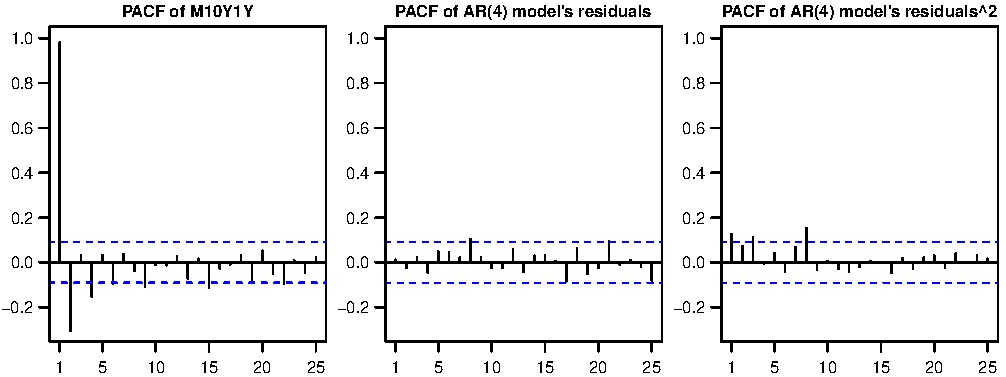
\includegraphics{figures/pacfplot.pdf}
  \caption{The sample partial autocorrelation function of the series \code{M10Y1Y} for the lags $1,...,25$ (on the right). The sample partial autocorrelation function of the Pearson residuals of a Gaussian AR($4$) model (on the middle) and of the squared residuals (on the right) for the lags $1,...,25$. The blue dashed lines are the $95\%$ critical bounds for partial autocorrelation coefficients of an IID process.}
\label{fig:pacf}
\end{figure}
%

Figure~\ref{fig:pacf} shows that the PACF of the series has very large partial autocorrelation coefficient (PACC) at the first lag, relatively large PACCs at the second and fourth lags, and visibly smaller PACCs after the fourth lag. The autoregressive order $p=4$ thereby seems a reasonable candidate for a parsimonious AR model.\footnote{It turns out that the order $p=4$ also minimizes the Akaike information criterion among the Gaussian AR($p$) models, $p=1,...,24$, based on the exact log-likelihood function (not shown).} Hence, we fitted a Gaussian AR($4$) model to the series and examined the PACF of its residuals and squared residuals, which are depicted in the middle and right panels of Figure~\ref{fig:pacf}, respectively.

The PACF of the AR($4$) model's residuals shows that there is not much autocorrelation left in the residuals, so the autoregressive order $p=4$ seems sufficient for capturing the autocorrelation structure of the series. The PACF of the AR($4$) model's squared residuals shows PACCs slightly outside the $95\%$ critical bounds at lags $1$, $3$, and $8$. Thereby the order $4$ could be somewhat sufficient for modelling the (potentially present) ARCH type conditional heteroskedasticity, but the order $9$ could also be considered for a less parsimonious model, as the lag $8$ PACC is relatively large. A StMAR model might, therefore, be appropriate with the autoregressive order $p=4$, although it may not be sufficient for modelling the conditional heteroskedasticity at larger lags. As discussed above, the two modes in the kernel density estimate of the series, on the other hand, indicate that two regimes seems like a good starting point for building the model.

If the candidate model is found inadequate, one may try to use a different autoregressive order $p$ or to add a regime to the model (or switch to the StMAR model, if a GMAR model is found inadequate). Note that while with linear AR models increasing the autoregressive order typically improves the fit, this is not necessarily the case with GSMAR models, as the autoregressive order affects the regime-switching dynamics. In particular, because the mixing weights (\ref{eq:alphamt}) are calculated using the whole joint distribution of the previous $p$ observations, with a small $p$, the regime-switching probabilities react more sensitively to individual observations than with a large $p$. It may hence be useful to also try to decrease the autoregressive order rather than just increase it.

In addition to comparing model adequacy (or forecasting accuracy, for example), information criteria can be utilized in the selection of the GSMAR model. \pkg{uGMAR} calculates the Akaike (AIC), Hannan-Quinn (HQIC), and Schwarz-Bayesian (BIC) information criteria. The values of the information criteria are not directly comparable for models with different autoregressive orders if estimation is based on the conditional log-likelihood function, as the numbers of observations used in estimation are different due to the different number of initial values. With the conditional log-likelihood function, the values of the information criteria can be divided by the number of observations used in the estimation (that is, the length of the series minus $p$) to obtain more comparable statistics. However, as the conditional estimation with each order $p$ is based on slightly different observations, the comparison should be done with caution. The exact log-likelihood function, in contrast, employs the full series in estimation and thereby yields comparable values of information criteria for models with different orders $p$.


\subsection{Examples of unconstrained estimation}\label{sec:example_estim}
\addcontentsline{toc}{subsection}{Examples of unconstrained estimation}

In this section, we demonstrate how to estimate GSMAR models with \pkg{uGMAR} and provide several examples in order to illustrate various frequently occurring situations. In addition to the ordinary estimation, we particularly show how a GSMAR model can be built based on a local-only maximum point when the ML estimate seems unreasonable (see Appendix~\ref{sec:simuexp}). We also consider the estimation of the appropriate G-StMAR model when the estimated StMAR model contains overly large degrees of freedom estimates \citep[see][Section 4]{Virolainen:2020}.

In \pkg{uGMAR}, the GSMAR models are defined as class \code{gsmar} S3 objects, which can be created with given parameter values using the constructor function \code{GSMAR} (see Section~\ref{sec:GSMAR}) or by using the estimation function \code{fitGSMAR}, which estimates the parameters and then builds the model. For estimation, \code{fitGSMAR} needs to be supplied with a univariate time series and the arguments specifying the model. The necessary arguments for specifying the model include the autoregressive order \code{p}, the number of mixture components \code{M}, and \code{model}, which should be either \code{"GMAR"}, \code{"StMAR"}, or \code{"G-StMAR"}. For GMAR and StMAR models, the argument \code{M} is a positive integer, whereas for the G-StMAR model it is a length two numeric vector specifying the number of GMAR type regimes in the first element and the number of StMAR type regimes in the second.

Additional arguments may be supplied to \code{fitGSMAR} in order to specify, for example, whether the exact log-likelihood function should be used instead of the conditional one (\code{conditional}), whether the model should be parametrized with the intercepts $\varphi_{m,0}$ or the regimewise unconditional means $\mu_m$ (\code{parametrization}), how many estimation rounds should be performed (\code{ncalls}), and how many central processing unit (CPU) cores should be used in the estimation (\code{ncores}). Some of the estimation rounds may end up in local-only maximum points or saddle points, but reliability of the estimation results can be improved by increasing the number of estimation rounds. A large number of estimation rounds may be required particularly when the number of mixture components is large, as the surface of the log-likelihood function becomes increasingly more challenging. It is also possible to adjust the settings of the genetic algorithm that is used to find the starting values. The available options are listed in the documentation of the function \code{GAfit} to which the arguments adjusting the settings will be passed.

It is also possible to automatically filter out inappropriate estimates by setting the argument \code{filter_estimates=TRUE} in \code{fitGSMAR}, which is the default option. In the following, the issue of these inappropriate solutions is discussed among other things. Therefore, this feature filtering out inappropriate solutions automatically is not utilized.

Section~\ref{sec:modelselection} concluded that a StMAR model with autoregressive order $p=4$ and $M=2$ mixture components seems like a reasonable candidate for modeling the monthly interest rate spread \code{M10Y1Y}. The following code fits this model to the series using the conditional log-likelihood function and performing 12 estimation rounds with eight CPU cores. The argument \code{seeds} supplies the seeds that initialize the random number generator at the beginning of each call to the genetic algorithm, thereby yielding reproducible results.
%
\begin{CodeChunk}
\begin{CodeInput}
R> fit42t <- fitGSMAR(M10Y1Y, p = 4, M = 2, model = "StMAR", conditional = TRUE,
+    ncalls = 10, ncores = 10, seeds = 1:10)
\end{CodeInput}
\begin{CodeOutput}
Using 10 cores for 10 estimation rounds...
Optimizing with a genetic algorithm...
  |++++++++++++++++++++++++++++++++++++++++++++++++++| 100% elapsed=04s
Results from the genetic algorithm:
The lowest loglik:  143.403
The mean loglik:    158.323
The largest loglik: 162.947
Optimizing with a variable metric algorithm...
  |++++++++++++++++++++++++++++++++++++++++++++++++++| 100% elapsed=01s
Results from the variable metric algorithm:
The lowest loglik:  178.46
The mean loglik:    180.683
The largest loglik: 184.846
Filtering inappropriate estimates...
Finished!
Warning message:
In warn_dfs(p = p, M = M, params = params, model = model) :
  The model contains overly large degrees of freedom parameter values.
  Consider switching to a G-StMAR model by setting the corresponding
  regimes to be GMAR type with the function 'stmar_to_gstmar'.
\end{CodeOutput}
\end{CodeChunk}
%
The progression of the estimation process is reported with a progress bar giving an estimate of the remaining estimation time. Also statistics on the spread of the log-likelihoods are printed after each estimation phase. The progress bars are generated during parallel computing with the package \pkg{pbapply} \citep{Solymos+Zawadzki:2020}.

The function throws a warning in the above example, because the model contains at least one very large degrees of freedom parameter estimate. Such estimates are warned about, because very large degrees of freedom parameters are redundant in the model and their weak identification might lead to numerical problems \citep[Section 4]{Virolainen:2020}. Specifically, overly large degrees of freedom parameter estimates may induce a nearly numerically singular Hessian matrix of the log-likelihood function when evaluated at the estimate, making the approximate standard errors and  \citeauthor{Kalliovirta:2012}'s (\citeyear{Kalliovirta:2012}) quantile residual tests often unavailable.

The estimates can be examined with the \code{print} method:
%
\begin{CodeChunk}
\begin{CodeInput}
R> fit42t
\end{CodeInput}
\begin{CodeOutput}
Model:
 StMAR, p = 4, M = 2, #parameters = 15, #observations = 468,
 conditional, intercept parametrization, not restricted, no constraints.

Regime 1
Mix weight: 0.81
Reg mean: 1.87
Var param: 0.04
Df param: 9.75

y = [0.06] + [1.28]y.1 + [-0.36]y.2 + [0.20]y.3 + [-0.15]y.4 + [sigma_mt]eps

Regime 2
Mix weight: 0.19
Reg mean: 0.55
Var param: 0.01
Df param: 9348.94

y = [0.04] + [1.34]y.1 + [-0.59]y.2 + [0.54]y.3 + [-0.36]y.4 + [sigma_mt]eps
\end{CodeOutput}
\end{CodeChunk}
%
The parameter estimates are reported for each mixture component separately so that the estimates can be easily interpreted. Each regime's autoregressive formula is presented in the form
\begin{equation}
y_t = \varphi_{m,0} + \varphi_{m,1}y_{t - 1} + ... + \varphi_{m,p}y_{t - p} + \sigma_{m,t}\varepsilon_{m,t}.
\end{equation}
The other statistics are listed above the formula, including the mixing weight pameter $\alpha_m$, the unconditional mean $\mu_m$, the variance parameter $\sigma_m^2$, and the degrees freedom parameter $\nu_m$. For GMAR type regimes (if any), $\sigma_{m,t}=\sigma_m$ so the estimate of the variance parameter $\sigma_m^2$ is reported directly in the autoregressive formula.

The above printout shows that the second regime's degrees of freedom parameter estimate is very large, which might induce numerical problems. However, since a StMAR model with some degrees of freedom parameters tending to infinity coincides with the G-StMAR model with the corresponding regimes switched to GMAR type, one may avoid the problems by switching to the appropriate G-StMAR model \citep[Section 4]{Virolainen:2020}. Switching to the appropriate G-StMAR model is recommended also because it removes the redundant degrees of freedom parameters from the model, thereby reducing its complexity. The function \code{stmar_to_gstmar} does this switch automatically by first removing the large degrees of freedom parameters and then estimating the G-StMAR model with a variable metric algorithm \citep[algorithm 21]{Nash:1990} using the induced parameter vector as the initial value.

To exemplify, the following code switches all the regimes of the StMAR model \code{fit42t} with a degrees of freedom parameter estimate larger than $100$ to GMAR type, and then estimates the corresponding G-StMAR model.
%
\begin{CodeChunk}
\begin{CodeInput}
R> fit42gs <- stmar_to_gstmar(fit42t, maxdf = 100)
\end{CodeInput}
\end{CodeChunk}
%
We use the \code{summary} method to obtain a more detailed printout of the estimated the G-StMAR model:
%
\begin{CodeChunk}
\begin{CodeInput}
R> summary(fit42gs, digits = 2)
\end{CodeInput}
\begin{CodeOutput}
Model:
 G-StMAR, p = 4, M1 = 1, M2 = 1, #parameters = 14, #observations = 468,
 conditional, intercept parametrization, not restricted, no constraints.

 log-likelihood: 182.35, AIC: -336.71, HQIC: -313.89, BIC: -278.75

Regime 1 (GMAR type)
Moduli of AR poly roots: 1.16, 1.45, 1.45, 1.16
Mix weight: 0.19 (0.09)
Reg mean: 0.55
Reg var:  0.14

y = [0.04] + [1.34]y.1 + [-0.59]y.2 + [0.54]y.3 + [-0.36]y.4 + sqrt[0.01]eps
    (0.01)   (0.10)       (0.20)      (0.19)       (0.12)          (0.00)

Regime 2 (StMAR type)
Moduli of AR poly roots: 1.07, 2.02, 2.02, 1.51
Mix weight: 0.81
Reg mean: 1.87
Var param: 0.04 (0.01)
Df param: 9.75 (4.17)
Reg var:  1.01

y = [0.06] + [1.28]y.1 + [-0.36]y.2 + [0.20]y.3 + [-0.15]y.4 + [sigma_mt]eps
    (0.02)   (0.05)       (0.09)      (0.09)       (0.06)

Process mean: 1.62
Process var:  1.11
First p autocors: 0.98 0.96 0.93 0.89
\end{CodeOutput}
\end{CodeChunk}
%
In the G-StMAR model, estimates for GMAR type regimes are reported before StMAR type regimes, in a decreasing order according to the mixing weight parameter estimates. As shown above, the model \code{fit42gs} incorporates one GMAR type regime and one StMAR type regime. The mixing weight parameter estimate $0.19$ of the GMAR type regime indicates that in the long run, roughly $19\%$ of the observations are generated from this regime. Estimates of the unconditional mean and variance ($0.55$ and $0.14$, respectively) are visibly smaller in the GMAR type regime than in the StMAR type regime ($1.87$ and $1.01$, respectively). Hence, the GMAR type seems to mostly account for the periods when the series takes smaller values and is less volatile, while the StMAR type regime covers the more volatile periods of larger values. Interestingly, the AR parameters are somewhat similar in both regimes, implying that it could be appropriate to restrict them to be identical (this will be tested in Section~\ref{sec:testconst}).

Approximate standard errors are given in parentheses under or next to the related estimates. Note that the last mixing weight parameter estimate does not have an approximate standard error because it is not parametrized. Likewise, there is no standard error for the intercepts if mean parametrization is used (by setting \code{parametrization = "mean"} in \code{fitGSMAR}) and vice versa. In order to obtain standard errors for the regimewise unconditional means or intercepts, one can easily swap between the mean and intercept parametrizations with the function \code{swap_parametrization}.

Missing values are reported when \pkg{uGMAR} is not able to calculate the standard error. This typically happens either because there is an overly large degrees of freedom parameter estimate in the model (as discussed above) or because the estimation algorithm did not stop a local maximum. In the latter case, the observed information matrix is not necessarily positive definite, implying that the diagonal entries of its inverse might not all be positive. Consequently, when extracting the approximate standard errors by taking the square roots of the diagonal entries from the inverse of the observed information matrix, the possibly present negative entries will lead to missing values.

Section~\ref{sec:examestim} discusses how to evaluate with \pkg{uGMAR} whether the estimate is a local maximum (and how to improve the reliability of it being the global maximum). If the estimate is not a local maximum, one may try running more iterations of the variable metric algorithm with the function \code{iterate_more}. However, often when the algorithm does not stop a local maximum, it stopped to an unreasonable point very near the boundary of parameter space. As will be discussed next, in such a case it might be more appropriate to consider an alternative estimate that is clearly in the interior of the parameter space.

Other statistics reported in the summary printout include the log-likelihood and values of the information criteria, the first and second moments of the process, as well as regime specific unconditional means, unconditional variances, and moduli of the roots of the AR polynomials $1-\sum_{i=1}^p\varphi_{m,i}z^i, \ m=1,...,M$. If some of the moduli are very close to one, the related estimates are near the boundary of the stationarity region. We demonstrate in Appendix~\ref{sec:simuexp} that when such solutions are accompanied with a very small variance parameter estimate, they might not be reasonable estimates and maximize the log-likelihood function for a technical reason only. Consequently, the estimate related to the next-largest local maximum could be considered.

This is possible in \pkg{uGMAR}, because the estimation function \code{fitGSMAR} stores the estimates from all the estimation rounds so that a GSMAR model can be built based on any one of them, most conveniently with the function \code{alt_gsmar}. The desired estimation round can be specified either with the argument \code{which_round} or \code{which_largest}. The former specifies the round in the estimation order, whereas the latter specifies it in a decreasing order of the log-likelihoods. To demonstrate this, we use the argument \code{filter_estimates=FALSE} in the following code to prevent the filtering of inappropriate estimates.

To give an example of a case where the estimates are very close the boundary of the stationarity region, we estimate the G-StMAR model directly with the following code.
%
\begin{CodeChunk}
\begin{CodeInput}
R> fit42gs2 <- fitGSMAR(M10Y1Y, p = 4, M = c(1, 1), model = "G-StMAR",
+    conditional = TRUE, ncalls = 16, ncores = 8, seeds = 72:87,
+    filter_estimates = FALSE)
\end{CodeInput}
\begin{CodeOutput}
Using 8 cores for 16 estimation rounds...
Optimizing with a genetic algorithm...
  |++++++++++++++++++++++++++++++++++++++++++++++++++| 100% elapsed=06s
Results from the genetic algorithm:
The lowest loglik:  140.441
The mean loglik:    155.421
The largest loglik: 167.858
Optimizing with a variable metric algorithm...
  |++++++++++++++++++++++++++++++++++++++++++++++++++| 100% elapsed=02s
Results from the variable metric algorithm:
The lowest loglik:  152.034
The mean loglik:    174.794
The largest loglik: 192.43
Finished!
Warning message:
In warn_ar_roots(ret) :
  Regime 1 has near-unit-roots! Consider building a model from the next-largest
  local maximum with the function 'alt_gsmar' by adjusting its argument
  'which_largest'.
\end{CodeOutput}
\end{CodeChunk}
%
The function throws a warning, because the largest found maximum point incorporates a regime that is very close to the boundary of the stationarity region, indicating that the estimate might be inappropriate.
We examine the estimates with the \code{summary} method:
%
\begin{CodeChunk}
\begin{CodeInput}
R> summary(fit42gs2, digits = 2)
\end{CodeInput}
\begin{CodeOutput}
Model:
 G-StMAR, p = 4, M1 = 1, M2 = 1, #parameters = 14, #observations = 468,
 conditional, intercept parametrization, not restricted, no constraints.

 log-likelihood: 192.43, AIC: -356.86, HQIC: -334.05, BIC: -298.90

Regime 1 (GMAR type)
Moduli of AR poly roots: 1.00, 1.00, 1.00, 1.00
Mix weight: 0.02 (0.03)
Reg mean: 2.65
Reg var:  0.13

y = [3.77] + [1.19]y.1 + [-1.81]y.2 + [1.19]y.3 + [-1.00]y.4 + sqrt[0.00]eps
    (0.02)   (0.01)       (0.01)      (0.01)       (0.00)          (0.00)

Regime 2 (StMAR type)
Moduli of AR poly roots: 1.04, 1.93, 1.93, 1.48
Mix weight: 0.98
Reg mean: 0.89
Var param: 0.04 (0.01)
Df param: 4.98 (1.67)
Reg var:  1.75

y = [0.02] + [1.30]y.1 + [-0.36]y.2 + [0.21]y.3 + [-0.17]y.4 + [sigma_mt]eps
    (0.01)   (0.05)       (0.08)      (0.08)       (0.05)

Process mean: 0.92
Process var:  1.78
First p autocors: 0.99 0.97 0.95 0.93
\end{CodeOutput}
\end{CodeChunk}
%
The summary statistics reveal that there are four near-unit-roots in the GMAR type regime and the variance parameter estimate is very small. Such estimates often occur when there are several regimes in the model and the estimation algorithm is ran a large number of times.

If one suspects that the estimate is inappropriate, it is easy to build a model based on the second-largest maximum point that was found in the estimation procedure. Below, the first line of the code builds the model based on the second-largest maximum point, and the second line calls the \code{summary} method to produce a detailed printout of the model.
%
\begin{CodeChunk}
\begin{CodeInput}
R> fit42gs3 <- alt_gsmar(fit42gs2, which_largest = 2)
R> summary(fit42gs3, digits = 2)
\end{CodeInput}
\begin{CodeOutput}
Model:
 G-StMAR, p = 4, M1 = 1, M2 = 1, #parameters = 14, #observations = 468,
 conditional, intercept parametrization, not restricted, no constraints.

 log-likelihood: 182.35, AIC: -336.71, HQIC: -313.89, BIC: -278.75

Regime 1 (GMAR type)
Moduli of AR poly roots: 1.16, 1.45, 1.45, 1.16
Mix weight: 0.19 (0.09)
Reg mean: 0.55
Reg var:  0.14

y = [0.04] + [1.34]y.1 + [-0.59]y.2 + [0.54]y.3 + [-0.36]y.4 + sqrt[0.01]eps
    (0.01)   (0.10)       (0.20)      (0.19)       (0.12)          (0.00)

Regime 2 (StMAR type)
Moduli of AR poly roots: 1.07, 2.02, 2.02, 1.51
Mix weight: 0.81
Reg mean: 1.87
Var param: 0.04 (0.01)
Df param: 9.75 (4.14)
Reg var:  1.01

y = [0.06] + [1.28]y.1 + [-0.36]y.2 + [0.20]y.3 + [-0.15]y.4 + [sigma_mt]eps
    (0.02)   (0.05)       (0.09)      (0.09)       (0.06)

Process mean: 1.62
Process var:  1.11
First p autocors: 0.98 0.96 0.93 0.89
\end{CodeOutput}
\end{CodeChunk}
%
The above printout shows that the estimates related to the second-largest local maximum are the same as of the model \code{fit42gs} (which was estimated based on a StMAR model with a very large degrees of freedom parameter estimate) and that they are clearly inside the stationarity region for all regimes. If also the second-largest maximum point seems unreasonable, a GSMAR model can be built based on the next-largest maximum point by adjusting the argument \code{which_largest} in the function \code{alt_gsmar} accordingly.

It is also possible to automatically filter out inappropriate estimates by setting the argument \code{filter_estimates=TRUE} in \code{fitGSMAR}, which is also the default option. Then, the function will automatically filter out estimates that it deems "inappropriate".  That is, estimates that are not likely solutions of interest. Specifically, it filters out solutions that incorporate regimes with any modulus of the roots of the AR polynomial less than $1.0015$; a variance parameter estimate near zero  (less than $0.0015$); mixing weights such that they are close to zero for almost all $t$ for at least one regime; or mixing weight parameterestimate close to zero (or one). You can also set \code{filter_estimates=FALSE} and find the solutions of interest yourself by using the function \code{alt_gsmar}. \code{fitGSMAR} then returns the solution based on the largest log-likelihood that is not filtered out. Other solutions can be studied by using the function \code{alt_gsmvar} as usual.


\subsection{Further examination of the estimates}\label{sec:examestim}
\addcontentsline{toc}{subsection}{Further examination of the estimates}

In addition to examining the summary printout, it is often useful to visualize the model by plotting the mixing weights together with the time series and the model's (marginal) stationary density together with a kernel density estimate of the time series. That is exactly what the plot method for GSMAR models does. For instance, the following command creates Figure~\ref{fig:fit42gs}:
%
\begin{CodeChunk}
\begin{CodeInput}
R> plot(fit42gs)
\end{CodeInput}
\end{CodeChunk}
%
As Figure~\ref{fig:fit42gs} (the top and bottom left panels) shows, the first regime prevails when the spread takes small values, while the second regime mainly dominates when the spread takes large values. The graph of the model's marginal stationary density (the right panel), on the other hand, shows that the two regimes capture the two modes in the marginal distribution of the spread. The hump shape in the right tail of the kernel density estimate is not explained by the mixture of the two distributions, but a third regime could be added for the purpose (for brevity, we do not study the three regime model further).

It is also sometimes interesting to examine the time series of (one-step) conditional means and variances of the process along with the time series the model was fitted to. This can be done conveniently with the function \code{cond_moment_plot}, where the argument \code{which_moment} should be specified with \code{"mean"} or \code{"variance"} accordingly. In addition to the conditional moment of the process, \code{cond_moment_plot} also displays the conditional means or variances of the regimes multiplied by the mixing weights. Note, however, that the conditional variance of the process is not generally the same as the weighted sum of regimewise conditional variances, as it includes a component that encapsulates heteroskedasticity caused by variation in the conditional mean \cite[see][Equation (2.19)]{Virolainen:2020}.

\begin{figure}[t]
  \centering
  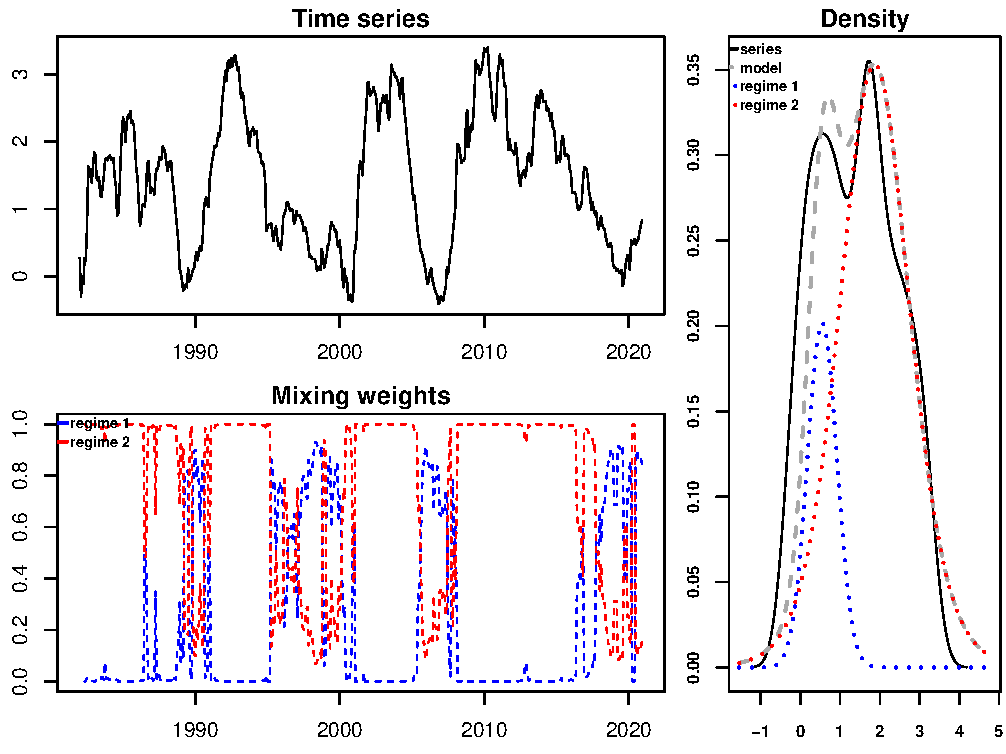
\includegraphics{figures/plotfit42gs.pdf}
  \caption{The figure produced by the command \code{plot(fit42gs)}. On the top left, the monthly spread between the 10-year and 1-year Treasury constant maturity rates, covering the period from 1982 January to 2020 December. On the bottom left, the estimated mixing weights of the G-StMAR model (\code{fit42gs}) fitted to the interest rate spread (blue dashed line for the first regime and red dashed line for the second regime). On the right, the one-dimensional marginal stationary density of the estimated G-StMAR model (grey dashed line) along with a kernel density estimate of the spread (black solid line) and marginal stationary densities of the regimes multiplied by the mixing weight parameter estimates (blue and red dotted lines).}
\label{fig:fit42gs}
\end{figure}

The variable metric algorithm employed in the final estimation does not necessarily stop at a local maximum point. The algorithm might also stop at a saddle point or near a local maximum, when the algorithm is not able to increase the log-likelihood, or at any point, when the maximum number of iterations has been reached. In the latter case, the estimation function throws a warning, but saddle points and inaccurate estimates need to be detected by the researcher.

It is well known that in a local maximum point, the gradient of the log-likelihood function is zero, and the eigenvalues of the Hessian matrix are all negative. In a local minimum, the eigenvalues of the Hessian matrix are all positive, whereas in a saddle point, some of them are positive and some negative. Nearly numerically singular Hessian matrices occur when the surface of the log-likelihood function is very flat about the estimate in some directions. This particularly happens when the model contains overly large degrees of freedom parameter estimates or the mixing weights $\alpha_{m,t}$ are estimated close to zero for all $t=1,...,T$ for some regime $m$.

\pkg{uGMAR} provides several functions for evaluating whether the estimate is a local maximum point. The function \code{get_foc} returns the (numerically approximated) gradient of the log-likelihood function evaluated at the estimate, and the function \code{get_soc} returns eigenvalues of the (numerically approximated) Hessian matrix of the log-likelihood function evaluated at the estimate. The numerical derivatives are calculated using a central difference approximation
\begin{equation}
\frac{\partial L(\boldsymbol{\theta})}{\partial \theta_i} \approx \frac{f(\boldsymbol{\theta} + \boldsymbol{h}^{(i)}) - f(\boldsymbol{\theta} - \boldsymbol{h}^{(i)})}{2h}, \ \ h>0,
\end{equation}
where $\theta_i$ is the $i$th element of $\boldsymbol{\theta}$ and $\boldsymbol{h}^{(i)}=(0,...,0,h,0,...,0)$
contains $h$ as its $i$th element. By default, the difference $h=6\cdot 10^{-6}$ is used for all parameters except for overly large degrees of freedom parameters, whose partial derivatives are approximated using larger differences. The difference is increased for large degrees of freedom parameters, because the limited precision of the float point presentation induces artificially rugged surfaces to the their profile log-likelihood functions, and the increased differences diminish the related numerical error. On the other hand, as the surface of the profile log-likelihood function is very flat about a large degrees of freedom parameter estimate, large differences work well for the approximation.

For example, the following code calculates the first order condition for the G-StMAR model \code{fit42gs}:
%
\begin{CodeChunk}
\begin{CodeInput}
R> get_foc(fit42gs)
\end{CodeInput}
\begin{CodeOutput}
 [1]  0.0576396128 -0.0364233988 -0.0242331476 -0.0144442609 -0.0161249574
 [6]  0.0411603528 -0.0171471584 -0.0490156277 -0.0659635759 -0.0587742714
[11] -0.0635655297  0.0686981920 -0.0374653647  0.0002778317
\end{CodeOutput}
\end{CodeChunk}
%
and the following code calculates the second order condition:
%
\begin{CodeChunk}
\begin{CodeInput}
R> get_soc(fit42gs)
\end{CodeInput}
\begin{CodeOutput}
 [1] -5.753554e-02 -1.354508e+01 -4.394382e+01 -6.467642e+01 -1.204519e+02
 [6] -1.672692e+02 -2.619181e+02 -8.869383e+02 -2.045380e+03 -4.862797e+03
[11] -4.355348e+04 -5.455077e+04 -2.727695e+05 -5.564824e+05
\end{CodeOutput}
\end{CodeChunk}
%
All eigenvalues of the Hessian matrix are negative, which points to a local maximum, but the gradient of the log-likelihood function seems to somewhat deviate from zero. The gradient might be inaccurate, because it is based on a numerical approximation. It is also possible that the estimate is inaccurate, because it is based on approximative numerical estimation, and the estimates are therefore not expected to be exactly accurate. Whether the estimate is a local maximum point with accuracy that is reasonable enough, can be evaluated by plotting the graphs of the profile log-likelihood functions about the estimate. In \pkg{uGMAR}, this can be done conveniently with the function \code{profile_logliks}.

The exemplify, the following command plots the graphs of profile log-likelihood functions of the estimated G-StMAR model \code{fit42gs}:
%
\begin{CodeChunk}
\begin{CodeInput}
R> profile_logliks(fit42gs, scale = 0.02, precision = 200)
\end{CodeInput}
\end{CodeChunk}
%
The output is displayed in Figure~\ref{fig:proflogfit42gs}, showing that the estimate's accuracy is reasonable, as changing any individual parameter value marginally would not visibly increase the log-likelihood. The argument \code{scale} can be adjusted to shorten or lengthen the interval shown in the horizontal axis. If one zooms in enough by setting \code{scale} to a very small number, it can be seen that the estimate is not exactly at the local maximum, but it is so close that moving there would not increase the log-likelihood notably. The argument \code{precision} can be adjusted to increase the number of points the graph is based on. For faster plotting, it can be decreased, and for more precision, it can be increased.

\begin{figure}[t]
  \centering
  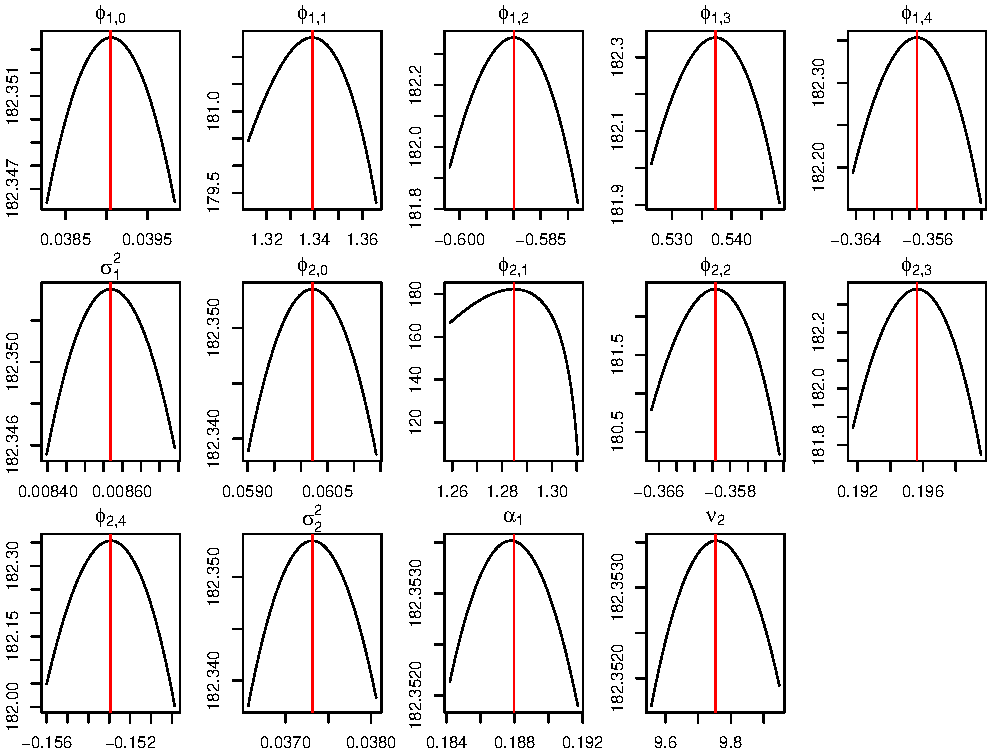
\includegraphics{figures/proflogfit42gs.pdf}
  \caption{The figure produced by the command \code{profile\_logliks(fit42gs)}. Graphs of the profile log-likelihood functions of the estimated G-StMAR model \code{fit42gs} with the red vertical lines pointing the estimates.}
\label{fig:proflogfit42gs}
\end{figure}

We have discussed tools that can be utilized to evaluate whether the found estimate is a local maximum with a reasonable accuracy. It is, however, more difficult to establish that the estimate is the global maximum. With \pkg{uGMAR}, the best way to increase the reliability that the found estimate is the global maximum, is to run more estimation rounds by adjusting the argument \code{ncalls} of the estimation function \code{fitGSMAR}. When a large number of estimation rounds is run (and $M>1$), \code{fitGSMAR} often finds peculiar near-the-boundary estimates that have extremely spiky profile log-likelihood functions for some parameters and are thus difficult to find (see Appendix~\ref{sec:simuexp}). Therefore, it seems plausible that \code{fitGSMAR} also finds a reasonable ML estimate with a good reliability.

\subsection{Examples of constrained estimation}\label{sec:examp_const}
\addcontentsline{toc}{subsection}{Examples of constrained estimation}

Alternatively to the unconstrained estimation, one may impose linear constraints on the autoregressive (AR) parameters of the model; that is, on $\varphi_{m,1},...,\varphi_{m,p}$, $m=1,...,M$. \pkg{uGMAR} deploys two types of constraints: the AR parameters can be restricted to be the same for all regimes and linear constraints can be applied to each regime separately. In order to impose the former type of constraints, the estimation function simply needs to be supplied with the argument \code{restricted = TRUE}.

For instance, the G-StMAR, $p=4$, $M_1=1$, $M_2=1$ model (\code{fit42gs}) estimated in Section~\ref{sec:example_estim} obtained somewhat similar estimates for the AR parameters in both regimes. The following code estimates a version of this model such that the AR parameters are restricted to be the same in both regimes. Note that this model still allows for shifts in the conditional (and unconditional) mean, as the intercept parameters can vary across the regimes. The argument \code{print_res = FALSE} tells \code{fitGSMAR} not to the print the spread of the log-likelihoods obtained from each phase of estimation.
%
\begin{CodeChunk}
\begin{CodeInput}
R> fit42gsr <- fitGSMAR(M10Y1Y, p = 4, M = c(1, 1), model = "G-StMAR",
+    restricted = TRUE, ncalls = 12, ncores = 8, seeds = 1:12,
+    print_res = FALSE)
\end{CodeInput}
\begin{CodeOutput}
Using 8 cores for 12 estimation rounds...
Optimizing with a genetic algorithm...
  |++++++++++++++++++++++++++++++++++++++++++++++++++| 100% elapsed=05s
Optimizing with a variable metric algorithm...
  |++++++++++++++++++++++++++++++++++++++++++++++++++| 100% elapsed=01s
Finished!
\end{CodeOutput}
\end{CodeChunk}
%
The summary printout of the model shows the AR parameter estimates are the same in both regimes:
%
\begin{CodeChunk}
\begin{CodeInput}
R> summary(fit42gsr)
\end{CodeInput}
\begin{CodeOutput}
Model:
 G-StMAR, p = 4, M1 = 1, M2 = 1, #parameters = 10, #observations = 468,
 conditional, intercept parametrization, AR parameters restricted, no
 constraints.

 log-likelihood: 180.02, AIC: -340.04, HQIC: -323.74, BIC: -298.64

Regime 1 (GMAR type)
Moduli of AR poly roots: 1.21, 1.83, 1.83, 1.21
Mix weight: 0.51 (0.17)
Reg mean: 2.13
Reg var:  0.46

y = [0.13] + [1.29]y.1 + [-0.40]y.2 + [0.25]y.3 + [-0.20]y.4 + sqrt[0.03]eps
    (0.03)   (0.05)       (0.08)      (0.08)       (0.05)          (0.00)

Regime 2 (StMAR type)
Moduli of AR poly roots: 1.21, 1.83, 1.83, 1.21
Mix weight: 0.49
Reg mean: 0.54
Var param: 0.05 (0.06)
Df param: 2.76 (1.18)
Reg var:  0.83

y = [0.03] + [1.29]y.1 + [-0.40]y.2 + [0.25]y.3 + [-0.20]y.4 + [sigma_mt]eps
    (0.01)   (0.05)       (0.08)      (0.08)       (0.05)

Process mean: 1.35
Process var:  1.27
First p autocors: 0.98 0.95 0.91 0.87
\end{CodeOutput}
\end{CodeChunk}
%
In constrast to the unrestricted model, this model has larger regimewise unconditonal mean in the GMAR type regime than in the StMAR type regime. According to the unconditional regimewise variances, the StMAR type regime is the more volatilite regime in this model as well.

Whether imposing the constraints is reasonable, can be evaluated by employing a statistical test, comparing values of the information criteria, or examining the model adequacy, for example. As the summary printout shows, the information criteria values all decreased as opposed to the unrestricted model, implying that the constraints could be appropriate. Discussion on testing the constraints is postponed to Section~\ref{sec:testconst}, whereas diagnostics checks for evaluating the model adequacy are covered in Section~\ref{sec:qres}.

The other type constraints in \pkg{uGMAR} are of the form
\begin{equation}
\boldsymbol{\varphi}_m = \boldsymbol{C}_m\boldsymbol{\psi}_m, \quad m=1,...,M,
\end{equation}
where $\boldsymbol{C}_m$ is a known $(p\times q_m)$ constraint matrix with full column rank, $\boldsymbol{\psi}_m$ is a $(q_m \times 1)$ parameter vector, and $\boldsymbol{\varphi}_m=(\varphi_{m,1},...,\varphi_{m,p})$ contains the AR coefficients of the $m$th regime. In order to apply the constraints, the estimation function should be supplied with the argument \code{constraints} containing a list of the constraint matrices $\boldsymbol{C}_m$, $m=1,...,M$.

To exemplify, consider a GMAR model with autoregressive order $p=3$ and $M=2$ mixture components. To constrain the third AR coefficient of the second regime ($\varphi_{2,3}$) to zero but leaving the first regime unconstrained, we deploy the following list of constraint matrices:
%
\begin{CodeChunk}
\begin{CodeInput}
R> C_list <- list(diag(3), matrix(c(1, 0, 0, 0, 1, 0), nrow = 3))
R> C_list
\end{CodeInput}
\begin{CodeOutput}
[[1]]
     [,1] [,2] [,3]
[1,]    1    0    0
[2,]    0    1    0
[3,]    0    0    1

[[2]]
     [,1] [,2]
[1,]    1    0
[2,]    0    1
[3,]    0    0
\end{CodeOutput}
\end{CodeChunk}
%
After setting up the constraints, the constrained model can be estimated as follows:
%
\begin{CodeChunk}
\begin{CodeInput}
R> fit32c <- fitGSMAR(M10Y1Y, p = 3, M = 2, model = "GMAR",
+    constraints = C_list, ncalls = 12, ncores = 8, seeds = 1:12,
+    print_res = FALSE)
\end{CodeInput}
\begin{CodeOutput}
Using 8 cores for 12 estimation rounds...
Optimizing with a genetic algorithm...
  |++++++++++++++++++++++++++++++++++++++++++++++++++| 100% elapsed=05s
Optimizing with a variable metric algorithm...
  |++++++++++++++++++++++++++++++++++++++++++++++++++| 100% elapsed=01s
Finished!
\end{CodeOutput}
\end{CodeChunk}
%
Printout of the model shows that the third AR parameter estimate of the second regime is zero:
%
\begin{CodeChunk}
\begin{CodeInput}
R> fit32c
\end{CodeInput}
\begin{CodeOutput}
Model:
 GMAR, p = 3, M = 2, #parameters = 10, #observations = 468,
 conditional, intercept parametrization, not restricted, linear constraints
 imposed.

Regime 1
Mix weight: 0.56
Reg mean: 1.26

y = [0.02] + [1.25]y.1 + [-0.19]y.2 + [-0.07]y.3 + sqrt[0.01]eps

Regime 2
Mix weight: 0.44
Reg mean: 1.72

y = [0.07] + [1.27]y.1 + [-0.32]y.2 + [0.00]y.3 + sqrt[0.05]eps
\end{CodeOutput}
\end{CodeChunk}
%
Notice that even when the $p$th AR coefficient is restricted to zero, the $p$th lag of that regime is accounted for in the mixing weights (\ref{eq:alphamt}) and in the case of a StMAR type regime also in the conditional variance (\ref{eq:sigmamt}).

If both types of constraints are applied at the same time, only a single constraint matrix should be supplied (not in a list). Consider a GSMAR model with $p=2$ and $M=2$, for example, and suppose the AR coefficients should be restricted to be the same in both regimes and the second AR coefficient ($\varphi_{m,2}$) should be constrained to be the negative of the first coefficient ($\varphi_{m,1}$). Then, the estimation function should be supplied with the arguments \code{restricted = TRUE} and \code{constraints = matrix(c(1, -1), nrow = 2)}. As demonstrated above, \pkg{uGMAR}'s implementation for applying linear constraints is not the most general one, but it makes applying some of the most typical constraints convenient, as the constraint matrices remain small.


\subsection{Testing parameter constraints}\label{sec:testconst}
\addcontentsline{toc}{subsection}{Testing parameter constraints}

One way to asses the validity of the imposed constraints is to compare the values of information criteria of the constrained and unconstrained models. \pkg{uGMAR}, however, also provides functions for testing the constraints with the likelihood ratio test and Wald test, which are applicable as the ML estimator of a GSMAR model has the conventional asymptotic distribution \cite[as long as the model is correctly specified and one is willing to assume the validity of the required unverified assumptions, see][pp. 254-255, \citealp{Meitz+Preve+Saikkonen:2021}, Theorem 3, and \citealp{Virolainen:2020}, Theorem 2]{Kalliovirta+Meitz+Saikkonen:2015}. For a discussion on the likelihood ratio and Wald tests, see \citet{Buse:1982} and the references therein, for example.

The likelihood ratio test considers the null hypothesis that the true parameter value $\boldsymbol{\theta}_0$ satisfies some constraints imposed on these parameters \cite[such that the constrained parameter space is a subset of the parameter space, which is presented in][Section 2.2 for the GSMAR models]{Virolainen:2020}. Denoting by $\hat{L}_U$ and $\hat{L}_C$ the (maximized) log-likelihoods based on the unconstrained and constrained ML estimates, respectively, the test statistic takes the form
\begin{equation}
LR=2(\hat{L}_U - \hat{L}_C).
\end{equation}
Under the null, the test statistic is asymptotically $\chi^2$-distributed with the degrees of freedom given by the difference in the dimensions of the unconstrained and constrained parameter spaces.

With \pkg{uGMAR}, the likelihood ratio test can be calculated with the function \code{LR_test}, which takes the unconstrained model (a class \code{gsmar} object) as its first argument and the constrained model as the second argument. For instance, in Section~\ref{sec:examp_const} we estimated a G-StMAR, $p=4$, $M_1=1$, $M_2=1$ model such that the AR parameters are restricted to be equal in both regimes (the model \code{fit42gsr}), i.e., $\boldsymbol{\varphi}_1=\boldsymbol{\varphi}_2$. The following code tests those constraints against the unconstrained model \code{fit42gs} with the likelihood ratio test and prints the results.
%
\begin{CodeChunk}
\begin{CodeInput}
R> LR_test(fit42gs, fit42gsr)
\end{CodeInput}
\begin{CodeOutput}
	Likelihood ratio test

data:  fit42gs and fit42gsr
LR = 4.6695, df = 4, p-value = 0.3229
alternative hypothesis: the true parameter does not satisfy the constraints
imposed in fit42gsr
\end{CodeOutput}
\end{CodeChunk}
%
The large $p$-value indicates that we cannot reject the constraints at any conventional level of significance, and it might thereby be reasonable to consider the constrained model if it is found adequate.

\pkg{uGMAR} implements the Wald test of the null hypothesis
\begin{equation}
A\boldsymbol{\theta}_0 = c,
\end{equation}
where $A$ is a $(k \times d)$ matrix with full row rank, $c$ is a $(k \times 1)$ vector, $\boldsymbol{\theta}_0$ is the true parameter value, $d$ is the dimension of the parameter space, and $k$ is the number of constraints. The Wald test statistic takes the form
\begin{equation}
W = (A\hat{\boldsymbol{\theta}} - c)'[A\mathcal{J}(\hat{\boldsymbol{\theta}})^{-1}A']^{-1}(A\hat{\boldsymbol{\theta}} - c),
\end{equation}
where $\mathcal{J}(\hat{\boldsymbol{\theta}})$ is the observed information matrix evaluated at the ML estimate $\hat{\boldsymbol{\theta}}$. Under the null, the test statistic is asymptotically $\chi^2$-distributed with $k$ degrees of freedom (which is the difference in dimensions of the constrained and unconstrained parameter spaces).

With \pkg{uGMAR}, the Wald test can be calculated with function \code{Wald_test}, which takes the estimated unconstrained model (as a class \code{gsmar} object) as the first argument, the matrix $A$ as the second argument, and the vector $c$ as the third argument. To exemplify, we test whether the AR parameters and intercepts are identical in both regimes of the G-StMAR, $p=4$, $M_1=1$, $M_2=1$ model, i.e., the null hypothesis $(\varphi_{1,0},\boldsymbol{\varphi}_1) = (\varphi_{2,0},\boldsymbol{\varphi}_2)$. %In this model, kurtosis and variance are still allowed to vary across the regimes.
The $(d \times 1)$ parameter vector $\boldsymbol{\theta}$ (which is presented at the end of Section~\ref{sec:gstmar} and again in Section~\ref{sec:GSMAR}) contains the intercept and AR parameters of the first regime in the entries $1,...,5$ and the intercept and AR parameters of the second regime in the entries $7,...,11$. The appropriate matrix $A$ and vector $c$ that state the hypothesis are set in the first two lines of the following code, and the third line calculates the test.
%
\begin{CodeChunk}
\begin{CodeInput}
R> c <- rep(0, times = 5)
R> A <- cbind(diag(5), c, -diag(5), c, c, c)
Wald_test(fit42gs, A = A, c = c)
\end{CodeInput}
\begin{CodeOutput}
	Wald test

data:  fit42gs, A, c
W = 15.107, df = 5, p-value = 0.009916
alternative hypothesis: the true parameter theta does not satisfy
A%*%theta = c
\end{CodeOutput}
\end{CodeChunk}
%

As the above printout shows, the $p$-value is small enough to reject the null at the $1\%$ level of significance, even though the null hypothesis that the AR parameters are equal in both regimes could not be rejected by the likelihood ratio test. Using the model \code{fit42gsr} to calculate a Wald test, that tests equality of the intercepts conditional on the constraint that the AR parameters are identical in both regimes, produces the $p$-value $0.00025$ (not shown for brevity). Thus, the intercepts are not likely equal if the AR parameters are identical in both regimes.\footnote{The test results do not, however, allow to infer that the process is likely bimodal, because GSMAR processes incorporating component processes with distinct means can have unimodal skewed marginal distributions. Moreover, one cannot infer about the (in)equality of the means of the component processes based on the (in)equality of the intercepts if the AR parameters are allowed vary freely. In particular, our null hypothesis $(\varphi_{1,0},\boldsymbol{\varphi}_1) = (\varphi_{2,0},\boldsymbol{\varphi}_2)$ does not test whether the component processes have identical means, as identical means can be obtained also with various other constraints. Identicality of the means can, however, be tested directly by switching to the mean parametrization (with the function \code{swap\_parametrization}) and calculating the appropriate Wald test.} As is demonstrated above, the Wald test has the benefit that it does not require estimation of the constrained model, and it is, therefore, not limited to the type of constraints \pkg{uGMAR} accommodates. The likelihood ratio test, on the other hand, is more conveniently calculated once the constrained model has been estimated.

Note that the standard tests are not applicable if the number of GMAR or StMAR type regimes is chosen too large, as then some of the parameters are not identified, causing the result of the asymptotic normality of the ML estimator to break down. This particularly happens when one tests for the number of regimes in the model, as under the null some of the regimes are reduced from the model\footnote{\cite{Meitz+Saikkonen:2021} have, however, recently developed such tests for mixture models with Gaussian conditional densities.} \citep[see the related discussion in][Section 3.3.2]{Kalliovirta+Meitz+Saikkonen:2015}. Similar caution applies for testing whether a regime is of the GMAR type against the alternative that it is of the StMAR type. Then $\nu_m = \infty$ under the null for the regime $m$ to be tested, which violates the assumption that the parameter value is in the interior of a compact subset of the parameter space \citep[see][Theorem 2 and Assumption 1]{Virolainen:2020}.


\section{Quantile residual based model diagnostics}\label{sec:qres}
\addcontentsline{toc}{section}{Quantile residual based model diagnostics}

In the GSMAR models, the empirical counterparts of the error terms $\varepsilon_{m,t}$ in (\ref{eq:defeq}) cannot be calculated, because the regime that generated each observation is unknown, making the conventional residual based diagnostics unavailable. Therefore, \pkg{uGMAR} utilizes so called \emph{quantile residuals}, which are suitable for evaluating adequacy of the GSMAR models. Deploying the framework presented in \cite{Kalliovirta:2012}, quantile residuals are defined as
%
\begin{equation}\label{eq:qres}
R_t=\Phi^{-1}(F(y_t|\mathcal{F}_{t-1})), \quad t=1,2,...,T,
\end{equation}
%
where $\Phi^{-1}(\cdot)$ is the standard normal quantile function and $F(\cdot|\mathcal{F}_{t-1})$ is the conditional cumulative distribution function of the considered GSMAR process (conditional on the previous observations). Closed form expressions for the quantile residuals of the GSMAR processes are derived in Appendix~\ref{sec:qresexpr}.
%

The empirical counterparts of the quantile residuals are calculated by using the parameter estimate and the observed data in (\ref{eq:qres}). For a correctly specified GSMAR model, the empirical counterparts of the quantile residuals based on the ML estimator are asymptotically independent with standard normal distributions \citep[Lemma 2.1]{Kalliovirta:2012}. Hence, quantile residuals can be used for graphical analysis similarly to the conventional Pearson residuals.

In \pkg{uGMAR}, quantile residuals can be analyzed graphically with the function \code{diagnostic_plot}, which plots the quantile residual time series, normal quantile-quantile plot, and sample autocorrelation functions of the quantile residuals and squared quantile residuals. If one sets \code{plot_indstats = TRUE} in the function arguments, \code{diagnostic_plot} also plots the standardized individual statistics discussed in \citet[pp. 369-370]{Kalliovirta:2012} with their approximate 95\% critical bounds.

The individual statistics, which test for remaining autocorrelation or heteroskestacity in specific lags, can be calculated either based on the observed data or based on the simulation procedure proposed by \cite{Kalliovirta:2012}. In the simulation procedure, the individual statistics' approximate standard errors are based on a sample simulated from the estimated process. According to \citeauthor{Kalliovirta:2012}'s (\citeyear{Kalliovirta:2012}) Monte Carlo study, the simulation procedure may improve size properties of the related tests, but it makes calculation of the statistics computationally more demanding - particularly if the simulated sample is very large.

The likelihood ratio test accepted hypothesis that the AR coefficients of the G-StMAR $p=4$, $M_1=1$, $M_2=2$ model are identical in both regimes (see Section~\ref{sec:testconst}). In order to evaluate whether this constrained model (\code{fit42gsr}) can adequately capture the autocorrelation structure, conditional heteroskedasticity, and distribution of the series, we create a diagnostic plot with the following code. We include \citeauthor{Kalliovirta:2012}'s (\citeyear{Kalliovirta:2012}) individual statistic to the figure based on the observed data and calculated for the first $20$ lags.
%
\begin{CodeChunk}
\begin{CodeInput}
R> diagnostic_plot(fit42gsr, nlags = 20, plot_indstats = TRUE)
\end{CodeInput}
\end{CodeChunk}
%

\begin{figure}[t]
  \centering
  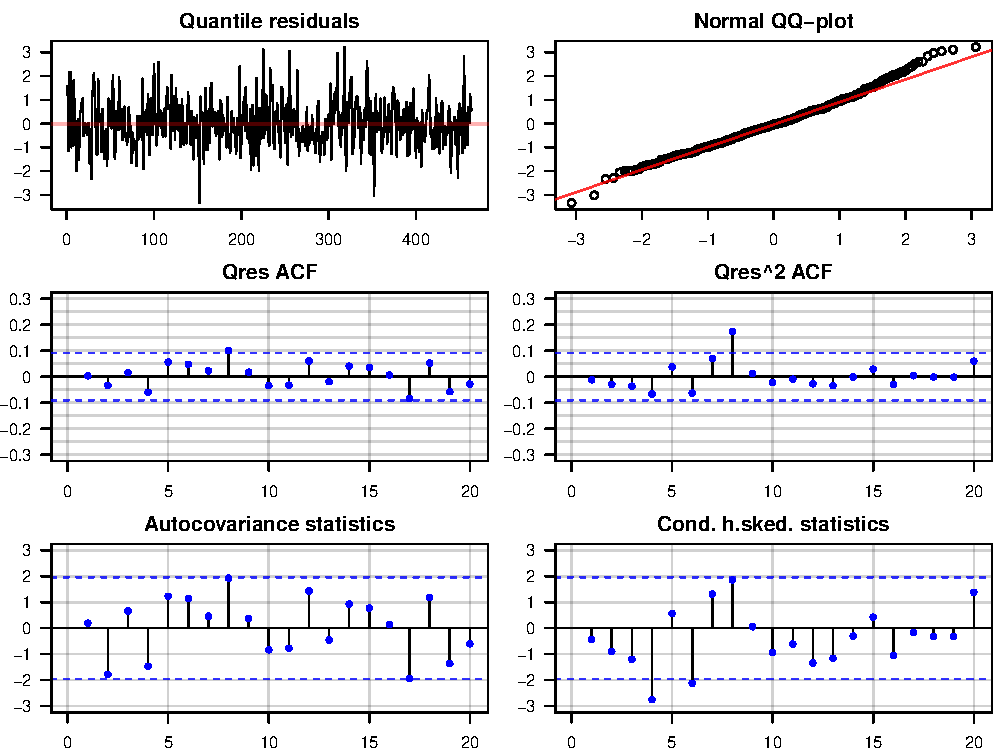
\includegraphics{figures/diagplotfit42gsr.pdf}
  \caption{Diagnostic plot for the fitted model \code{fit42gsr} created using the function \code{diagnostic\_plot}. The quantile residual time series (top left), normal  quantile-quantile plot (top right), sample autocorrelation functions of the quantile residuals (middle left) and squared quantile residuals (middle right), and the individual autocorrelation (bottom left) and heteroskedasticity (bottom right) statistics discussed in \citet[pp. 369-370]{Kalliovirta:2012}. The blue dashed lines in the sample autocorrelation figures are the $1.96T^{-1/2}$ lines denoting 95\% critical bounds for IID-observations, whereas for \citeauthor{Kalliovirta:2012}'s (\citeyear{Kalliovirta:2012}) individual statistics they are the approximate 95\% critical bounds.}
\label{fig:diagplotfit42gs}
\end{figure}

The resulting plot is presented in Figure~\ref{fig:diagplotfit42gs}. The quantile residual time series (the top left panel) has a period when it takes several consecutive negative values (roughly the observations $260,...,300$ with also some positive observations in between), but other than that it seems to somewhat resemble an IID normal process. The normal quantile-quantile plot (the top right panel) shows that the quantile residuals' distribution has too fat right tail. This is possibly due to the inability to explain the hump shape in the right tail of the series' distribution with a mixture of one normal and one $t$-distribution, when the two modes are accounted for.

The sample autocorrelation function of the quantile residuals (the middle left panel) shows that there are no particularly large autocorrelation coefficients in the lags $1,...,20$. Moreover, as all \citeauthor{Kalliovirta:2012}'s (\citeyear{Kalliovirta:2012}) autocorrelation statistics fall inside the asymptotic $95\%$ critical bounds, the model seems to adequately describe the autocorrelation structure of the series. The sample autocorrelation function of the squared quantile residuals (the middle right panel), on the other hand, has a relatively large coefficient at the lag eight. \citeauthor{Kalliovirta:2012}'s (\citeyear{Kalliovirta:2012}) conditional heteroskedasticity statistics (the bottom right panel) fall outside the asymptotic $95\%$ critical bounds at the lags four and six, but at the lag eight the statistic is inside the bounds. Overall, it appears that in addition to the distribution, the model might not adequately explain the conditional heteroskedasticity of the series.

In order to employ the simulation procedure for calculating the individual statistics, one needs to set the length of the simulated sample with the argument \code{nsimu}. If \code{nsimu} is not larger than the length of the observed data, the statistics will be based on the observed data. In addition to \code{diagnostic_plot}, quantile residuals can be graphically examined with the function \code{quantile_residual_plot}, which plots the quantile residual time series and a histogram.

Analyzing quantile residuals graphically gives an overview of the model's adequacy, but it is often appealing to also carry out a formal testing procedure. \cite{Kalliovirta:2012} proposes three specific tests for testing normality,  autocorrelation, and conditional heteroskedasticity of the quantile residuals. \citeauthor{Kalliovirta:2012}'s (\citeyear{Kalliovirta:2012}) tests take into account the uncertainty caused by estimation of the parameters and they are shown to perform well in a simulation study \citep[Section 4]{Kalliovirta:2012}.

In \pkg{uGMAR}, the quantile residual tests can be applied with the function \code{quantile_residual_tests} whose arguments include the model and the numbers of lags to be included in the autocorrelation (\code{lags_ac}) and heteroskedasticity tests  (\code{lags_ch}). Similarly to the individual statistics discussed in the context of the diagnostic plot, the tests can be based either on the observed data or on the simulation procedure. The simulation procedure can be deployed by setting the argument \code{nsimu} to be larger than the data length.

The following code calculates the quantile residual tests for the restricted G-StMAR model \code{fit42gsr} by deploying the simulation procedure based on a simulated sample of length $10000$ and taking into account $1,3,6$, and $12$ lags in the autocorrelation and heteroskedasticity tests. By default, the lags for the heteroskedasticity tests are the same as for the autocorrelation tests, so it is enough to set the autocorrelation test lags with the argument \code{lags_ac}.
%
\begin{CodeChunk}
\begin{CodeInput}
R> set.seed(1)
R> qrtr <- quantile_residual_tests(fit42gsr, lags_ac = c(1, 3, 6, 12),
+    nsimu = 10000)
\end{CodeInput}
\begin{CodeOutput}
Normality test p-value: 0.018

Autocorrelation tests:
lags | p-value
  1  |  0.849
  3  |  0.084
  6  |  0.488
  12 |  0.213

Conditional heteroskedasticity tests:
lags | p-value
  1  |  0.713
  3  |  0.299
  6  |  0.017
  12 |  0.000
\end{CodeOutput}
\end{CodeChunk}
%
The test results reveal that the model does not seem to adequately capture the conditional heteroskedasticity in the series when taking into account $12$ lags. Also, the normality test and the heteroskedasticity test with six lags pass only at $1\%$ level of significance. The rest of the tests, including all the autocorrelation tests pass at $5\%$ level of significance, confirming our findings from examining the diagnostic plot: the model seem to adequately explain the autocorrelation structure of the series but struggles in capturing the distribution and conditional heteroskedasticity. Nevertheless, the inadequacies do not seem very serious.

Because the restricted model was found somewhat inadequate, we run the quantile residual tests for the unrestricted model as well in order to evaluate whether it captures the statistical properties of the series more adequately. The following code runs the same diagnostics tests for the unrestricted model \code{fit42gs}.
%
\begin{CodeChunk}
\begin{CodeInput}
R> set.seed(1)
R> qrt <- quantile_residual_tests(fit42gs, lags_ac = c(1, 3, 6, 12),
+    nsimu = 10000)
\end{CodeInput}
\begin{CodeOutput}
Normality test p-value: 0.087

Autocorrelation tests:
lags | p-value
  1  |  0.475
  3  |  0.020
  6  |  0.289
  12 |  0.077

Conditional heteroskedasticity tests:
lags | p-value
  1  |  0.579
  3  |  0.137
  6  |  0.002
  12 |  0.000
\end{CodeOutput}
\end{CodeChunk}
%
As the $p$-values show, relaxing the restrictions improved the model's capability to capture the distribution of the series but according to the test results, the unrestricted model does not explain conditional heteroskedasticity as well as the restricted one when taking into account six lags (since the test now rejects at $1\%$ level of significance). Also the autocorrelation test with three lags only passes at $1\%$ level of significance. It thereby appears that the parsimonious restricted model could be more appropriate. Adding a third regime to the model or trying a different autoregressive order could also be considered for potentially improving the adequacy.

\pkg{uGMAR} often fails to calculate the quantile residual tests for GSMAR models with very large degrees of freedom parameter estimates, but the problem can be avoided by switching to the appropriate G-StMAR model with the function \code{stmar_to_gstmar}, which removes the redundant degrees of freedom parameters \citep[see][Section 4, and Section~\ref{sec:example_estim} of this paper]{Virolainen:2020}. Calculation of the tests may also fail when the estimate is very close to the boundary of the parameter space in which case it might be appropriate to consider an estimate from the next-largest local maximum point of the log-likelihood function. To that end, the function \code{alt_gsmar} can be used as demonstrated in Section~\ref{sec:example_estim} and in Appendix~\ref{sec:simuexp}.


\section{Building a GSMAR model with specific parameter values}\label{sec:GSMAR}
\addcontentsline{toc}{section}{Building a GSMAR model with specific parameter values}

The function \code{GSMAR} facilitates building GSMAR models without estimation, for instance, in order to simulate observations from a GSMAR process with specific parameter values. The parameter vector (of length $M(p+3)+M_2-1$ for unconstrained models) has the form $\boldsymbol{\theta} = (\boldsymbol{\vartheta}_1,...,\boldsymbol{\vartheta}_M,\alpha_1,...,\alpha_{M-1},\boldsymbol{\nu})$ where
\begin{align}
\boldsymbol{\vartheta}_m &= (\varphi_{m,0},\varphi_{m,1},...,\varphi_{m,p},\sigma^2_m),\ \ m=1,...,M, \ \text{and}  \\
\boldsymbol{\nu} &= (\nu_{M_1+1},...,\nu_M).
\end{align}
%
In the GMAR model (when $M_1=M$), the vector $\boldsymbol{\nu}$ is omitted, as the GMAR model does not contain degrees of freedom parameters. For models with constraints on the autoregressive parameters, the parameter vectors are expressed in a different way. For brevity, they are only presented in the package documentation, because the hand-specified parameter values can be set to satisfy any constraints as is.

In addition to the parameter vector, \code{GSMAR} should be supplied with arguments \code{p} and \code{M} specifying the order of the model similarly to the estimation function \code{fitGSMAR} discussed in Sections \ref{sec:example_estim} and \ref{sec:examp_const}. If one wishes to parametrize the model with the regimewise unconditional means ($\mu_m$) instead of the intercepts ($\varphi_{m,0}$), the argument \code{parametrization} should be set to \code{"mean"} in which case the intercept parameters $\varphi_{m,0}$ are replaced with $\mu_m$ in the parameter vector. By default, \pkg{uGMAR} uses intercept parametrization.

To exemplify, we build the GMAR $p=2$, $M=2$ model that is used in the simulation experiment in Appendix~\ref{sec:simuexp}. The model has intercept parametrization and parameter values $\boldsymbol{\vartheta}_1 = (0.9, 0.4, 0.2, 0.5)$, $\boldsymbol{\vartheta}_2 = (0.7, 0.5, -0.2, 0.7)$, and $\alpha_1 = 0.7$. After building the model, we use the \code{print} method to examine it:
%
\begin{CodeChunk}
\begin{CodeInput}
R> params22 <- c(0.9, 0.4, 0.2, 0.5, 0.7, 0.5, -0.2, 0.7, 0.7)
R> mod22 <- GSMAR(p = 2, M = 2, params = params22, model = "GMAR")
R> mod22
\end{CodeInput}
\begin{CodeOutput}
Model:
 GMAR, p = 2, M = 2, #parameters = 9,
 conditional, intercept parametrization, not restricted, no constraints.

Regime 1
Mix weight: 0.70
Reg mean: 2.25

y = [0.90] + [0.40]y.1 + [0.20]y.2 + sqrt[0.50]eps

Regime 2
Mix weight: 0.30
Reg mean: 1.00

y = [0.70] + [0.50]y.1 + [-0.20]y.2 + sqrt[0.70]eps
\end{CodeOutput}
\end{CodeChunk}
%

It is possible to include data in the models built with \code{GSMAR} by either providing the data in the argument \code{data} when creating the model or by adding the data afterwards with the function \code{add_data}. When the model is supplied with data, the mixing weights, one-step conditional means and variances, and quantile residuals can be calculated and included in the model. The function \code{add_data} can also be used to update data to an estimated GSMAR model without re-estimating the model.


\section{Simulation and forecasting}\label{sec:simufore}
\addcontentsline{toc}{section}{Simulation and forecasting}

\subsection{Simulation}\label{sec:simu}
\addcontentsline{toc}{subsection}{Simulation}

\pkg{uGMAR} implements the S3 method \code{simulate} for simulating observations from GSMAR processes. The method requires the process to be given as a class \code{gsmar} object, which are typically created either by estimating a model with the function \code{fitGSMAR} or by specifying the parameter values by hand and building the model with the constructor function \code{GSMAR}. The initial values required to simulate the first $p$ observations can be either set by hand (with the argument \code{init_values}) or drawn from the stationary distribution of the process (by default). The argument \code{nsim} sets the length of the sample path to be simulated.

To give an example, the following code sets the random number generator seed to one and simulates the 500 observations long sample path that is used in the simulation experiment in Appendix~\ref{sec:simuexp} from the GMAR process built in Section~\ref{sec:GSMAR}:
%
\begin{CodeChunk}
\begin{CodeInput}
R> mysim <- simulate(mod22, nsim = 500, seed = 1)
\end{CodeInput}
\end{CodeChunk}
%
Our implementation of \code{simulate} returns a list containing the simulated sample path in \code{\$sample}, the mixture component that generated each observation in \code{\$component}, and the mixing weights in \code{\$mixing_weights}.

\subsection{Simulation based forecasting}
\addcontentsline{toc}{subsection}{Simulation based forecasting}

Deriving multiple-steps-ahead point predictions and prediction intervals analytically for the GSMAR models is very complicated, so \pkg{uGMAR} employs the following simulation-based method. By using the last $p$ observations of the data up to the date of forecasting as initial values, a large number of sample paths for the future values of the process are simulated. Then, sample quantiles from the simulated sample paths are calculated to obtain prediction intervals, and the median or mean is used for point predictions. A similar procedure is also applied to forecast future values of the mixing weights, which might be of interest because the researcher can often associate specific characteristics to different regimes.

Forecasting is most conveniently done with the \code{predict} method. The available arguments include the number of steps ahead to be predicted (\code{n_ahead}), the number sample paths the forecast is based on (\code{nsimu}), possibly multiple confidence levels for prediction intervals (\code{pi}), prediction type (\code{pred_type}), and prediction interval type (\code{pi_type}). The prediction type can be either \code{median}, \code{mean}, or for one-step-ahead forecasts also the exact conditional mean, \code{cond_mean}. The prediction interval type can be any of \code{"two-sided"}, \code{"upper"}, \code{"lower"}, or \code{"none"}.

\begin{figure}[t]
  \centering
  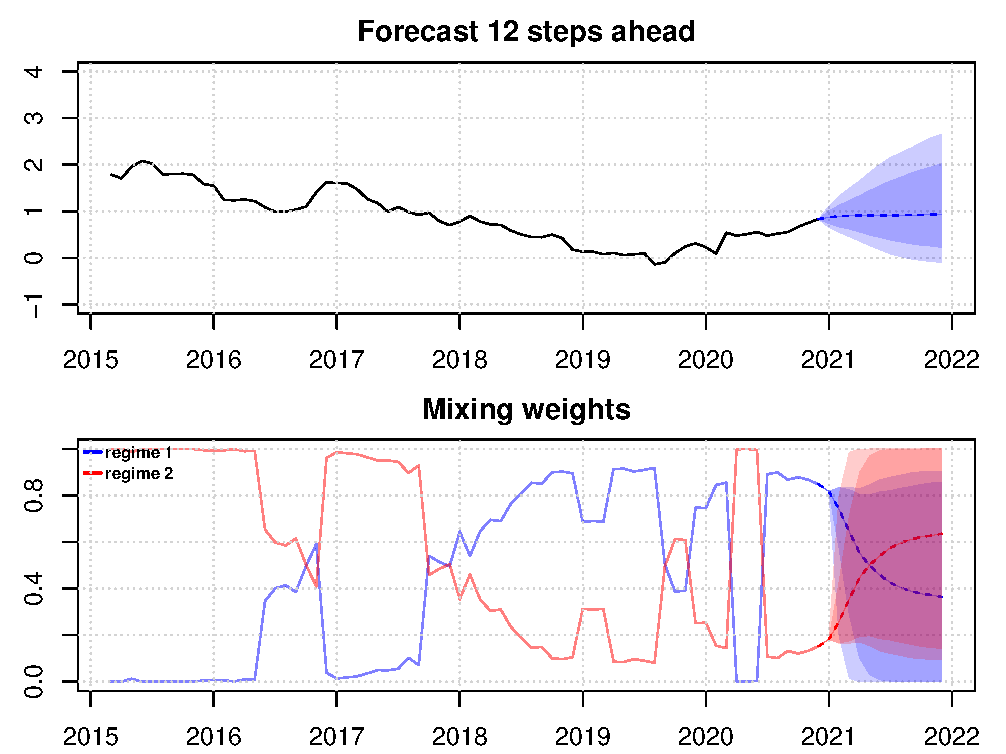
\includegraphics{figures/predictfit42gs.pdf}
  \caption{The figure created by the \code{predict} method for the G-StMAR model \code{fit42gs}. Twelve-months-ahead point prediction for the monthly interest rate spread (top) and the model's mixing weights (bottom) together with several preceding observations and prediction intervals with confidence levels $0.95$ (outer interval) and $0.80$ (inner interval).}
\label{fig:predictfit42gs}
\end{figure}

As an example, we use the unrestricted G-StMAR $p=4, M_1=1, M_2=1$ model fitted to the monthly interest rate spread in Section \ref{sec:example_estim} to forecast the spread $12$ months ahead, i.e., for the year 2021. The point prediction is based on median and $10000$ simulated future sample paths, and the two-sided prediction intervals are calculated for the confidence levels $0.95$ and $0.80$.
%
\begin{CodeChunk}
\begin{CodeInput}
R> set.seed(1)
R> mypred <- predict(fit42gs, n_ahead = 12, nsimu = 10000,
+    pi = c(0.95, 0.8), pred_type = "median", pi_type = "two-sided")
R> mypred
\end{CodeInput}
\begin{CodeOutput}
Prediction by median, two-sided prediction intervals with levels 0.95, 0.8.
Forecast 12 steps ahead, based on 10000 simulations.

   0.025  0.1 median  0.9 0.975
1   0.66 0.74   0.87 1.00  1.11
2   0.55 0.66   0.89 1.13  1.32
3   0.46 0.62   0.90 1.23  1.49
4   0.36 0.56   0.91 1.33  1.65
5   0.26 0.49   0.91 1.45  1.83
6   0.17 0.44   0.91 1.55  2.01
7   0.09 0.38   0.91 1.65  2.15
8   0.02 0.34   0.91 1.73  2.26
9  -0.02 0.30   0.92 1.82  2.36
10 -0.05 0.27   0.92 1.89  2.47
11 -0.08 0.25   0.93 1.95  2.58
12 -0.10 0.23   0.93 2.02  2.65

Point forecasts and prediction intervals for mixing weights can be obtained
with $mix_pred and $mix_pred_ints, respectively.
\end{CodeOutput}
\end{CodeChunk}

The \code{predict} method plots the results by default, but plotting can be also avoided by setting \code{plot_res = FALSE} in the arguments. The results can be plotted afterwards by using the \code{plot} method for the class \code{gsmarpred} objects that the \code{predict} method returns.

The figure created by the above example is presented in Figure~\ref{fig:predictfit42gs}. The point forecast does not predict any significant movements for the spread, but the prediction intervals appear to be skewed to the right. A possible explanation to the skewed prediction intervals is that at time of forecasting, the spread takes a value that is closer to the mean of the low-mean first regime than to the mean of the high-mean second regime. Hence, even if the process proceeds in the first regime, it does not (on average) move much lower, but switching to the second regime would (on average) lead to notably larger observations. Also, the forecast for the mixing weights reveals that after a few months, the high-mean second regime is predicted to become more probable than than the low-mean first regime, thus, explaining the skewed prediction intervals.


\section{Summary}\label{sec:summary}
\addcontentsline{toc}{section}{Summary}

Mixture autoregressive models are useful for analyzing time series that exhibit nonlinear, regime-switching features. The GMAR model, the StMAR model, and the G-StMAR model constitute an appealing family of such models, the GSMAR models, with attractive theoretical and practical properties. This paper introduced the \proglang{R} package \pkg{uGMAR} providing a comprehensive set of easy-to-use tools for GSMAR modeling, including unconstrained and constrained maximum likelihood estimation of the model parameters, quantile residual based model diagnostics, simulation, forecasting, and more. For convenience, we have collected some useful functions in \pkg{uGMAR} to Table~\ref{tab:functions}.

The model parameters are estimated with the method of maximum likelihood by employing a two-phase procedure, which uses a genetic algorithm to find starting values for a variable metric algorithm. Notably, due to the endogenously determined mixing weights, the maximum likelihood estimate is occasionally found very close to the boundary of the stationarity region of some regimes. We explained in Appendix~\ref{sec:simuexp} why such estimates might be inappropriate and showed how a GSMAR model can be built based on an alternative estimate related to the next-largest local maximum point.


\section*{Computational details}
\addcontentsline{toc}{section}{Computational details}

%The results in this paper were obtained using \proglang{R}~4.1.2 and \pkg{uGMAR}~3.4.1 package running on MacBook Pro 14", 2021, with Apple M1 Pro processor, 16 Gt of unified RAM, and macOS Monterey 12.1 operating system.

\pkg{uGMAR} takes use of the \proglang{R} package \pkg{Brobdingnag} \citep{Hankin:2007} to handle values extremely close to zero in the evaluation of the first term of the exact log-likelihood function (\ref{eq:loglik}). The package \pkg{gsl} \citep{Hankin:2006} is utilized to calculate some of the quantile residuals (\ref{eq:qres}) with a hypergeometric function. In order to improve computational efficiency in the numerical estimation procedure, the formula proposed by \cite{Galbraith+Galbraith:1974} is utilized to directly compute the inverses of the covariance matrices $\boldsymbol{\Gamma}_m$, $m=1,...,M$, (which appear in (\ref{eq:sigmamt}), (\ref{eq:dm}), (\ref{eq:alphamt}), and in the first term of (\ref{eq:loglik})), as only the inverses are required for calculating the quantities in the log-likelihood function. Finally, the algorithm proposed by \cite{Monahan:1984} is employed to generate random stationary autoregressive coefficients in the genetic algorithm.

Some of the estimation results (and thereby everything that is calculated based on the estimates) may vary slightly when running the code on different computers. This is due to a small numerical error in the gradient of the log-likelihood function caused by the limited precision of the floating-point representation. The negligible numerical error accumulates in each iteration of the variable metric algorithm, which hence advances in slightly different paths on different computers (with given initial values). After a large number of iterations, the algorithm might therefore end up in slightly different points. This particularly occurs when there are StMAR type regimes in the model, possibly because there are many different pairs of degrees of freedom and variance parameter values that are relatively close to each other and yield almost the same log-likelihoods.


\section*{Acknowledgments}
\addcontentsline{toc}{section}{Acknowledgments}

The author thanks Markku Lanne, Mika Meitz, and Pentti Saikkonen from comments and discussions, which helped to improve this paper substantially. The author also thanks Academy of Finland for financing the project (grant 308628).


\cleardoublepage
\section*{A table of some useful functions}\label{sec:table}
\addcontentsline{toc}{section}{A table of some useful functions}

\begin{table}[!h]
\centering
\begin{tabular}{llp{6.9cm}}
\hline
Related to     & Name                      & Description \\ \hline
Estimation     & \code{fitGSMAR}           & Estimate a GSMAR model.\\
               & \code{alt_gsmar}          & Build a GSMAR model based on results from any estimation round.\\
               & \code{stmar_to_gstmar}    & Estimate a G-StMAR model based on a StMAR (or G-StMAR) model with large degrees of freedom parameters.\\
               & \code{iterate_more}       & Run more iterations of the variable metric algorithm for a preliminary estimated GSMAR model.\\
Estimates      & \code{summary} (method)   & Detailed printout of the estimates.\\
               & \code{plot} (method)      & Plot the series with the estimated mixing weights and a kernel density estimate of the series with the stationary density of the model.\\
               & \code{get_foc}            & Calculate numerically approximated gradient of the log-likelihood function evaluated at the estimate.\\
               & \code{get_soc}            & Calculate eigenvalues of numerically approximated Hessian of the log-likelihood function evaluated at the estimate.\\
               & \code{profile_logliks}    & Plot the graphs of the profile log-likelihood functions.\\
               & \code{cond_moment_plot}   & Plot the model implied one-step conditional means or variances.\\
Diagnostics    & \code{quantile_residual_tests} & Calculate quantile residual tests.\\
               & \code{diagnostic_plot}    & Plot quantile residual diagnostics.\\
               & \code{quantile_residual_plot}  & Plot quantile residual time series and histogram.\\
Forecasting    & \code{predict} (method)   & Forecast future observations and mixing weights of the process.\\
Simulation     & \code{simulate} (method)  & Simulate from a GSMAR process.\\
Create model   & \code{GSMAR}              & Construct a GSMAR model based on specific parameter values.\\
Hypothesis testing & \code{LR_test}        & Calculate likelihood ratio test.\\
               & \code{Wald_test}          & Calculate Wald test.\\
Other          & \code{add_data}           & Add data to a GSMAR model \\
               & \code{swap_parametrization} & Swap between mean and intercept parametrizations \\
\hline
\end{tabular}
\caption{Some useful functions in \pkg{uGMAR} sorted according to their usage. The note "method" in parentheses after the name of a function signifies that it is an S3 method for a class \code{gsmar} object (often generated by the function \code{fitGSMAR} or \code{GSMAR}).}
\label{tab:functions}
\end{table}


\pagebreak
\bibliography{refs}

\newpage

\begin{appendix}

\section{Simulation experiment}\label{sec:simuexp}
\addcontentsline{toc}{section}{Appendix A: Simulation experiment}

This simulation experiment demonstrates why the log-likelihood function's global maximum point, that is found very near the boundary of the parameter space, might not be a reasonable estimate and why it might be more appropriate to consider a local-only maximum point that is clearly in the interior of the parameter space. We generated $500$ observations from a GMAR $p=2$‚ $M=2$ process with the parameter values given in the first row of Table~\ref{tab:simuexp} ($\boldsymbol{\theta}$) and initial values generated from the stationary distribution of the process. This model is built with \pkg{uGMAR} as an example in Section~\ref{sec:GSMAR}, and the sample path is generated as an example in Section~\ref{sec:simu}.

We estimated a GMAR $p=2$‚ $M=2$ model to the generated sample based on the exact log-likelihood function by performing $100$ estimation rounds using the following code (output is omitted for brevity):
%
\begin{CodeChunk}
\begin{CodeInput}
R> fit22 <- fitGSMAR(mysim$sample, p = 2, M = 2, model = "GMAR",
+    conditional = FALSE, ncalls = 100, ncores = 8, seeds = 1:100)
\end{CodeInput}
\end{CodeChunk}
%$
The obtained estimates are reported on the second row of Table~\ref{tab:simuexp} ($\hat{\boldsymbol{\theta}}_1$) together with the moduli of each regime's AR polynomial's ($1-\sum_{i=1}^p \varphi_{m,i}z^i$) roots. The modulus of the $i$th root in the $m$th regime is denoted by the symbol $\xi_{m,i}$. The stationarity condition requires that all the moduli are strictly greater than one, so the second regime is very close to the boundary of the stationarity region (both roots are approximately $1.000011$). Also the variance parameter $\sigma_2^2$ is close to its lower bound zero (it is approximately $9\cdot 10^{-6}$).

\begin{table}[p]
\centering
\begin{tabular}{c c c c c c c c c c c c c c} %{llp{9.2cm}}
\hline
    & $\varphi_{1,0}$ & $\varphi_{1,1}$ & $\varphi_{1,2}$ & $\sigma_1^2$ & $\varphi_{2,0}$ & $\varphi_{2,1}$ & $\varphi_{2,2}$ & $\sigma_2^2$ & $\alpha_1$ & $\xi_{1,1}$ & $\xi_{1,2}$ & $\xi_{2,1}$ & $\xi_{2,2}$\\
\hline
$\boldsymbol{\theta}$ & $0.90$ & $0.40$ & $0.20$ & $0.50$ & $0.70$ & $0.50$ & $-0.20$ & $0.70$ & $0.70$ & $1.45$ & $3.45$ & $2.24$ & $2.24$ \\
$\hat{\boldsymbol{\theta}}_1$ & $0.58$ & $0.56$ & $0.10$ & $0.61$ & $7.85$ & $-1.67$ & $-1.00$ & $0.00$ & $0.99$ & $1.42$ & $6.86$ & $1.00$ & $1.00$ \\
$\hat{\boldsymbol{\theta}}_2$ & $1.16$ & $0.39$ & $0.08$ & $0.54$ & $0.77$ & $0.35$ & $-0.17$ & $0.53$ & $0.63$ & $1.86$ & $6.90$ & $2.42$ & $2.42$ \\
\hline
\end{tabular}
\caption{On the first row, the true parameter values of the GMAR $p=2$, $M=2$ process that generated the sample path used in the simulation experiment. On the second row, the estimates that maximized the log-likelihood function based $100$ estimation rounds. On the third row, the estimates from the largest such log-likelihood function's maximum point that is not very near the boundary of the stationarity region. In each row after the estimates or parameter values, the moduli of the related AR polynomial's roots are presented.}
\label{tab:simuexp}
\end{table}

\begin{figure}[p]
  \centering
  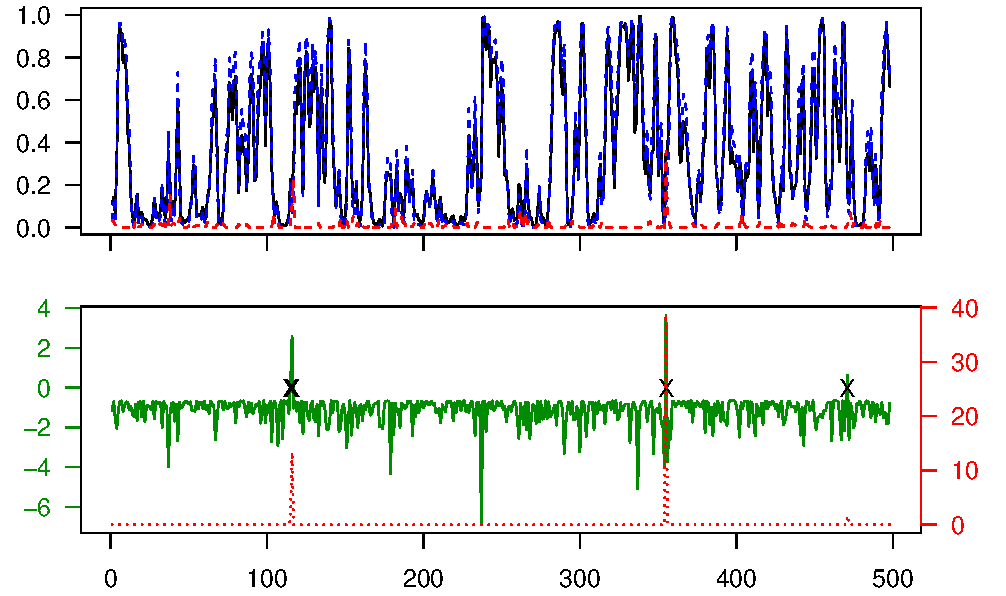
\includegraphics{figures/figsimuexp.pdf}
  \caption{On the top, the GMAR $p=2$, $M=2$ process's second regime's true mixing weights (black solid line), the mixing weights based on the estimate $\hat{\boldsymbol{\theta}}_1$ in the second row of Table~\ref{tab:simuexp} (red dashed line), and the mixing weights based on the estimate $\hat{\boldsymbol{\theta}}_2$ in the third row of Table~\ref{tab:simuexp} (blue dashed line). On the bottom, the terms (\ref{eq:loglik2}) from the second term of the log-likelihood function (\ref{eq:loglik}) (green solid line) and the second regime's densities in the terms (\ref{eq:loglik2}) multiplied by the estimated mixing weights (blue dotted line), i.e., $\alpha_{2,t}n_1(y_t;\mu_{2,t},\sigma_2^2)$, both based on the estimate $\hat{\boldsymbol{\theta}}_1$. The "X"-symbols denote the points where the second regime's conditional mean for the model based on estimate $\hat{\boldsymbol{\theta}}_1$ deviates from the corresponding observation by less than $0.005$.}
\label{fig:simuexp}
\end{figure}

These estimates produce a large log-likelihood, because the second regime's very small conditional variance makes the related density function in the term $l_t(\boldsymbol{\theta})$ (\ref{eq:loglik2}) to take large values near its mean, and the strong conditional mean targets individual observations there. This is illustrated in Figure~\ref{fig:simuexp} (bottom panel), where the terms $l_t(\boldsymbol{\theta})$ are presented (green solid line) together with the second regime's related weighted densities $\alpha_{2,t}n_1(y_t;\mu_{2,t},\sigma_2^2)$ (red dotted line). The black "X"-symbols denote the points where the second regime's conditional mean deviates from the corresponding observation by less than $0.005$. Evidently, the second regime contributes to the log-likelihood function only in the individual points where both, the terms $l_t(\boldsymbol{\theta})$ and the scaled densities $\alpha_{2,t}n_1(y_t;\mu_{2,t},\sigma_2^2)$, take large values due to the observation being close to the mean of the second regime's spikelike conditional density function. Because the scaled densities take large enough values in those individual points, the log-likelihood is larger for this kind of estimate than for a reasonable estimate.

The top panel of Figure~\ref{fig:simuexp} presents the true mixing weights of the GMAR process's second regime (black solid line) together with the mixing weights based on the estimate $\hat{\boldsymbol{\theta}}_1$ (red dashed line). As the figure shows, the estimated mixing weights are spiky and have no resemblance to the true mixing weights. Although the true mixing weights can be spiky for some GSMAR processes, spiking mixing weights are also typical for potentially inappropriate near-the-boundary estimates.

This kind of near-the-boundary estimates are often found when a subset of the regimes explains the variation in the series reasonably well, leaving some of the regimes available for targeting individual observations with very small conditional variance and very strong conditional mean. As such estimates seem to maximize the log-likelihood function for a technical reason, and not necessarily because they represent a good guess for the true parameter value, it might be appropriate to consider an alternative estimate related to the next-largest local maximum point. To exemplify, we build a model based on the largest local maximum point that is clearly in the interior of the parameter space. In our estimation based on $100$ rounds of the two-phase procedure, such an estimate is found at the point that induced the third largest log-likelihood, and it is obtained as follows:
%
\begin{CodeChunk}
\begin{CodeInput}
R> fit22_alt <- alt_gsmar(fit22, which_largest = 3)
\end{CodeInput}
\end{CodeChunk}
%
The corresponding estimate is presented on the third row of Table~\ref{tab:simuexp} ($\hat{\boldsymbol{\theta}}_2$). This local maximum point is substantially closer to the true parameter value in the second regime. The resemblance to the true parameter value is also highlighted in Figure~\ref{fig:simuexp} (top panel), where the second regime's estimated mixing weights (blue dashed line) are presented together with the true mixing weights (black solid line).

Finally, observe that the estimate $\hat{\boldsymbol{\theta}}_1$ presented in Table~\ref{tab:simuexp} is not the accurate maximum likelihood estimate, which can be noticed by examining graphs of the related profile log-likelihood functions with the command \code{profile_logliks(fit22)} (not shown). The numerical estimation using numerical approximation for the gradient of the log-likelihood function can be inaccurate near the boundary of a multidimensional parameter space subject to several constraints. Consequently, other similar near-the-boundary points that induce larger log-likelihood than $\hat{\boldsymbol{\theta}}_1$ can be found by running more estimation rounds. It should also be noted that sometimes the estimate is near the boundary of the stationarity region because the series is very persistent, and being near the boundary does not hence necessarily imply that the MLE is inappropriate.

\section{Closed form expressions of quantile residuals}\label{sec:qresexpr}
\addcontentsline{toc}{section}{Appendix B: Closed form expressions of quantile residuals}

This section derives closed form expressions for the quantile residuals utilized by \pkg{uGMAR} and discussed in Section~\ref{sec:qres}. For the GSMAR models, the quantile residuals are defined as
%
\begin{equation}\label{eq:qres1}
R_t=\Phi^{-1}(F(y_t|\mathcal{F}_{t-1})), \quad t=1,2,...,T,
\end{equation}
%
where $\Phi^{-1}(\cdot)$ is the standard normal quantile function,
%
\begin{equation}\label{eq:condcum}
F(y_t|\mathcal{F}_{t-1})= \sum_{m=1}^M\alpha_{m,t}\int_{-\infty}^{y_t} f_m(u_t|\mathcal{F}_{t-1})du_t
\end{equation}
%
is the conditional cumulative distribution function of the considered GSMAR process (conditional on the previous observations),
and $f_m(\cdot|\mathcal{F}_{t-1})$ is the conditional density function of the $m$th component process. To find a closed form expression for the quantile residuals defined in (\ref{eq:qres1}) and (\ref{eq:condcum}), it therefore suffices to solve the integrals $\int_{-\infty}^{y_t} f_m(u_t|\mathcal{F}_{t-1})du_t$, $m=1,...,M$, for GMAR type and StMAR type mixture components.
%

In the case of a GMAR type component, the conditional density function is the Gaussian density function with mean $\mu_{m,t}$ and variance $\sigma_m^2$. For $m\leq M_1$ in (\ref{eq:condcum}), we therefore have
%
\begin{equation}
\int_{-\infty}^{y_t} f_m(u_t|\mathcal{F}_{t-1})du_t = \int_{-\infty}^{y_t}n_1(u_t;\mu_{m,t},\sigma_m^2) du_t= \Phi\left(\frac{u_t - \mu_{m,t}}{\sigma_m}\right),
\end{equation}
%
where $\Phi (\cdot)$ is the standard normal cumulative distribution function.

In the case of a StMAR type component, the conditional density function is the Student's $t$ density function with mean $\mu_{m,t}$, variance $\sigma_{m,t}^2$, and $\nu_m + p$ degrees of freedom given as \cite[Appendix A]{Meitz+Preve+Saikkonen:2021}
%
\begin{equation}
t_1(u_t;\mu_{m,t},\sigma_{m,t}^2,\nu_m+p) = \frac{\Gamma\left(\frac{1 + \nu_m + p}{2}\right)}{\sqrt{\pi(\nu_m + p - 2)}\Gamma\left(\frac{\nu_m + p}{2}\right)}\sigma_{m,t}^{-1}\left(1 + \frac{(u_t - \mu_{m,t})^2}{(\nu_m + p - 2)\sigma_{m,t}^2} \right)^{-(1 + \nu_m + p)/2}
\end{equation}
%
where $\Gamma\left(\cdot\right)$ is the gamma function. Taking use of the symmetry of the Student's $t$ distribution about its mean $\mu_{m,t}$, we obtain
%
\begin{equation}\label{eq:int1}
\int_{-\infty}^{y_t} f_m(u_t|\mathcal{F}_{t-1})du_t = \frac{1}{2} + \int_{\mu_{m,t}}^{y_t}t_1(u_t;\mu_{m,t},\sigma_{m,t}^2,\nu_m+p) du_t.
\end{equation}
%

By applying the change of variables $\tilde{u}_{m,t}\equiv u_t - \mu_{m,t}$ in the integral, the right side of (\ref{eq:int1}) can be expressed as
%
\begin{equation}\label{eq:int2}
\frac{1}{2} + \frac{\Gamma\left(\frac{1 + \nu_m + p}{2}\right)}{\sqrt{\pi(\nu_m + p - 2)}\Gamma\left(\frac{\nu_m + p}{2}\right)}\sigma_{m,t}^{-1} \int_{0}^{\tilde{y}_{m,t}}\left(1 + \frac{\tilde{u}_{m,t}^2}{a_{m,t}} \right)^{-b_m} d \tilde{u}_{m,t},
\end{equation}
%
where $\tilde{y}_{m,t} \equiv y_t - \mu_{m,t}$, $a_{m,t}\equiv (\nu_m + p - 2)\sigma_{m,t}^2$, and $b_{m}\equiv (1 + \nu_m + p)/2$. Then, by applying the change of variables $z_{m,t}\equiv \tilde{u}_{m,t}^2/\tilde{y}_{m,t}$, we can express the integral in the expression (\ref{eq:int2}) as
%
\begin{equation}\label{eq:int3}
\int_{0}^{\tilde{y}_{m,t}}\left(1 + \frac{\tilde{u}_{m,t}^2}{a_{m,t}} \right)^{-b_m} d \tilde{u}_{m,t} = \frac{1}{2} \int_{0}^{\tilde{y}_{m,t}} \left(\frac{\tilde{y}_{m,t}}{z_{m,t}}\right)^{1/2}\left(1 + \frac{z_{m,t}\tilde{y}_{m,t}}{a_{m,t}}\right)^{-b_m}d z_{m,t}.
\end{equation}
%
By applying the third change of variables $x_{m,t}\equiv z_{m,t}/\tilde{y}_{m,t}$ and using the properties of the gamma function, the right side of (\ref{eq:int3}) can be expressed using a hypergeometric function as
%
\begin{equation}
\frac{\tilde{y}_{m,t}}{2}\int_{0}^{1}x_{m,t}^{-1/2}\left(1-x_{m,t}\left(-\frac{\tilde{y}_{m,t}^2}{a_{m,t}} \right) \right)^{-b_{m}} dx_{m,t}=\tilde{y}_{m,t} \times {}_2\text{F}_1\left(\frac{1}{2},b_{m},\frac{3}{2};-\frac{\tilde{y}_{m,t}^2}{a_{m,t}} \right),
\end{equation}
%
where the hypergeometric function is defined as \citep[Section 1.3.1]{Aomoto+Kita:2011}
\begin{equation}
{}_2\text{F}_1\left(a,b,c;x \right) = \frac{\Gamma(c)}{\Gamma(a)\Gamma(c-a)}\int_{0}^{1}s^{a-1}(1-s)^{c-a-1}(1-sx)^{-b} ds,
\end{equation}
when $|x|<1$, $a>0$, and $c-a>0$ (when $a,c\in\mathbb{R}$).

Using the above result, we have
\begin{equation}\label{eq:int4}
\int_{-\infty}^{y_t} f_m(u_t|\mathcal{F}_{t-1}) = \frac{1}{2} + \frac{\Gamma\left(\frac{1 + \nu_m + p}{2}\right)}{\sqrt{\pi(\nu_m + p - 2)}\Gamma\left(\frac{\nu_m + p}{2}\right)}\sigma_{m,t}^{-1} \tilde{y}_{m,t} \times {}_2\text{F}_1\left(\frac{1}{2},b_{m},\frac{3}{2};-\frac{\tilde{y}_{m,t}^2}{a_{m,t}}\right)
\end{equation}
for $m>M_1$, whenever $\left|-\frac{\tilde{y}_{m,t}^2}{a_{m,t}}\right|<1$. That is, the closed form expression (\ref{eq:int4}) exists when
\begin{equation}\label{eq:qrescond}
|y_t - \mu_{m,t}| < \sqrt{(\nu_m + p - 2)\sigma_{m,t}^2}.
\end{equation}
If this condition does not hold, \pkg{uGMAR} calculates the quantile residual by numerically integrating the conditional density function $f_m(\cdot|\mathcal{F}_{t-1})$.
\end{appendix}


\end{document}
